\chapter{Analysis}
\label{chap:analysis}
	As is to be expected, solutions for solving the problem already exist. In this chapter these solutions are investigated and evaluated, as to how well they solve the problem at hand. While finding solutions that match the problem described in  \emph{completely} might be difficult, solutions that are fairly similar are also considered.

	Furthermore, available academic research papers will be studied, for solutions that would solve a problem similar to that in \ref{chap:intro_sec:problem}, or a interesting techniques for handling sub-problems.

	\section{Existing Available Tools}
		Having several available tools which -- more or less -- \emph{could} be used to solve the problems, the findings have been condensed into the following list.
		\begin{itemize}
			\item In-Browser Password Managers
			\item LastPass, and Similar Solutions
			\item KeePass, and Similar Solutions
			\item Rattic
			\item Encryptr
			\item Passwordstate
			\item Vault \emph{(Zoho)}
			\item TeamPasswordManager
			\item Simple Safe
			\item PassWork
			\item SimpleVault
			\item RoboForm
			\item TeamPass 
			\item Vaultier
			%\item Vault (https://vaultproject.io/)
		\end{itemize}
		In the following sections the user experience or the usability of the solution might seem to be attacked often. While this might be true, one simple fact remains: If the solution is not user friendly, the users will not use it. If they do not use the solution, it is effectively worthless.

		\subsection*{In-Browser Password Managers}
			\label{subsec:in-browser}
			\todo{Write section about in-password managers}
			\todo{Missing browsers: Chrome, Firefox, Safari, IE, Opera}

			The most used password manager of all times, is probably the one available to all: The password manager which is built-in into the various browsers. This is a feature most major browsers have adopted: Chrome, FireFox, Internet Explorer \emph{(now known as Edge)}, Safari and Opera.

			While all of the previously mentioned browsers support syncing \emph{(Internet Explorer only supports this using Windows 8.0 or newer.)} the passwords between devices, it requires to upload the passwords to one of the corporations websites.

			Additionally it lacks at one very important aspect: It only works for websites accessed through that \emph{specific} type of browser, i.e. only available in Chrome browsers. Passwords for email addresses  \emph{(assuming non-webmail)} for instance, wont be able to be easily retrieved. Already at this point, using the built-in password manager can be dismissed, simply due to its use cases.

			In \cite{browser_saved} they review the different browsers' storage format for their respective password managers. Their primary concern is, that while the passwords might be encrypted, both Firefox and Opera stores the decryption key directly on disk. If an attacker gets hold of this file, all passwords are available to him or her. Chrome and Safari, however, use Window's built in functions, and encrypts the files using the user accounts password for encryption. They note Firefox and Opera as the only browsers supporting a Master Password, which is to be entered every time the user accesses a password stored, which adds a bit of more security. However, their analysis could very well be deprecated by now. The version of Chrome, for instance, they're using is $V21.0$, while the current newest version is $V47.0$. 

			While this solution might seem interesting to some users, it still leaves a lot to be desired in regards to the requirements defined earlier.

		\subsection*{LastPass, and Similar Solutions}
			\label{subsec:lastpass}
			In the name of usability services such as LastPass\footnote{https://lastpass.com/}, PassPack\footnote{https://www.passpack.com/}, DashLane\footnote{https://www.dashlane.com/}, and so many others grew popular, and it is easy to understand why. Enabling you to access your passwords from several devices, through native apps or the browser, it seemed like it was the perfect match of usability and security. To avoid too much repetition LastPass is picked as a representative of this group, simply due to it being the most well-known.

			If we start by looking at the technical details of LastPass, they quote themselves using 256-bit AES encryption, and applies PBKDF2, in order to make it as difficult as possible, to crack stored data. For maximum security, both encryption and decryption, is done client side\cite{lastpass_cleintsideencryption}, as to avoid transferring the actual password, unencrypted, to their servers. Encryption and decryption is done using the master password, which is never actually sent to their servers. Finally, as is to be expected, all connections to LastPass' servers, are SSL encrypted.

			Having examined the technical aspect, we need to pay attention to the usability as well. Looking at their web UI, it shows a reasonably straight forward design. Allowing the user to organise passwords folders, creating a two-level structure, as seen on figure \ref{fig:lastpass_main} on page \pageref{fig:lastpass_main}. While this \emph{does} allow the user some level of organisation, several levels would have been preferable. Additionally, LastPass is renowned for their apps and plugins, covering all major operating systems and browsers, creating a near seamless integration, when it comes to addition of new passwords and auto-filling stored passwords.

			For devices without a browser supporting plugins, LastPass offers a so-called bookmarklet\cite{lastpass_bookmarklet}. A bookmarklet is a bookmark, which essentially contains JavaScript code, in order to add previously unobtainable features, in a browser. While this on the surface seems like a nifty feature, several studies have shown that the bookmarklets represent a significant security threat. In \cite{bookmarklet} they discuss an attack on LastPass, exploiting the users bookmarklet, to gain access to virtually all of the users stored credentials.

			However, with the recent leak from LastPass \cite{lastpass_leak}, more and more users grew suspicious of these services. No matter how much encryption you apply, you can not get around the fact, that you have to \emph{trust} LastPass to both be completely honest about their encryption technology, \emph{and} storing your sensitive data. In many of the more sceptical user's eyes, this is a huge drawback, and why this solution is deemed unusable to solve the problem at hand.


			\begin{figure}[h!]
				\centering
				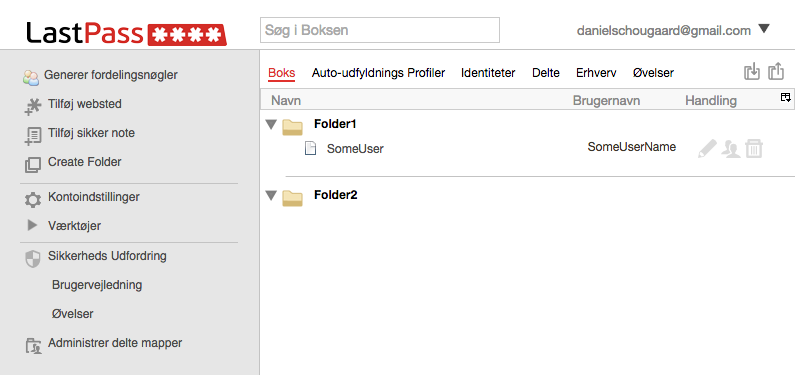
\includegraphics[width=\textwidth]{figures/analysis/lastpass_main.png}
				\caption{Screenshot of LastPass' main view, in a browser.}
				\label{fig:lastpass_main}
			\end{figure}

		\subsection*{KeePass}
			As the users grew suspicious of LastPass and the likes, a lot of them moved over to e.g. KeePass\footnote{https://keepass.org}, which allows the user to store the passwords in a local file. While there exists a plethora of tools similar to KeePass,  it will be used as a representative of this group, for the same reasons as in \ref{subsec:lastpass}.

			If we again start by examining the technical details, as of version 2.x KeePass only -- per default -- offers AES-256 encryption, which is seen on figure \ref{fig:keepass_create_security} on page \pageref{fig:keepass_create_security}, with additional algorithm choices available through plugins \cite{keepass_security}. This enables users to tailor the encryption security, to their own needs -- and beliefs. 

			Looking at the main UI, of which an example is shown on figure \ref{fig:keepass_main} on page \pageref{fig:keepass_main}, KeePass features exactly that which could be improved in LastPass: A tree like structure, in order to completely organise passwords. Other than that, there isn't anything noteworthy to say about their UI: It features the necessary and that's about it. A final thing worth mentioning, is that their password generator is completely customisable, as seen on figure \ref{fig:keepass_newpassword_passwordgen} on page \pageref{fig:keepass_newpassword_passwordgen}. You can manually choose, exactly which character sets, you wish to be in your passwords, enabling you to have passwords using local accents should the target system support it, which is a really nifty feature.


			However, having praised the features of KeePass, it does lack something extremely important: Usability. More precisely, it lacks distribution. Since KeePass works on a local file, it would only inherently work on a \emph{single} device. Should one wish to distribute it, another tool has to be involved. File synchronisation tools, such as Dropbox, Google Drive, or Syncthing could be used, in order to create a distributed-ish feel to KeePass. However, you do still rely on a third party tool, which is a drawback. Additionally, there is the lack of cross-platform compatibility, since \emph{officially} KeePass only supports Windows. Granted, there exists unofficial ports for Linux, OS X, Android, etc., but you have to trust the developers of these unofficial applications. By extension, this introduces the threat of security breaches. Another negative in regards to usability, is the lack of a browser extension. While there exists third party solutions for this, the authors personal experiences with setting these up and using them, is \emph{quite} negative.	

			Hence, all things taken into consideration, while KeePass has its moments it is an less than ideal solution.

			
			\begin{figure}[h!]
				\centering
				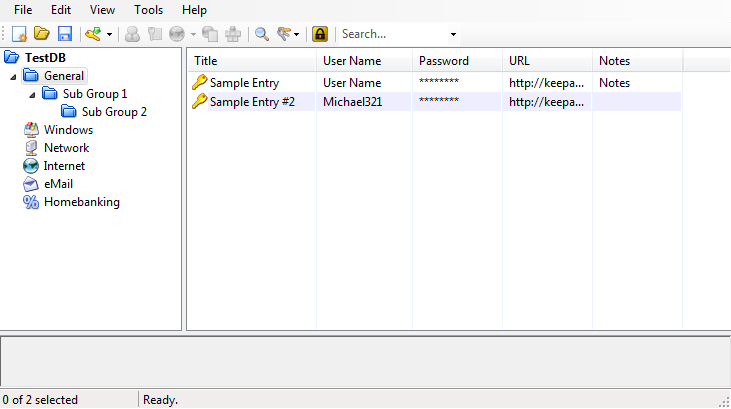
\includegraphics[width=\textwidth]{figures/analysis/keepass_mainview.png}
				\caption{Screenshot of KeePass' main view.}
				\label{fig:keepass_main}
			\end{figure}

			\begin{figure}[h!]
				\centering
				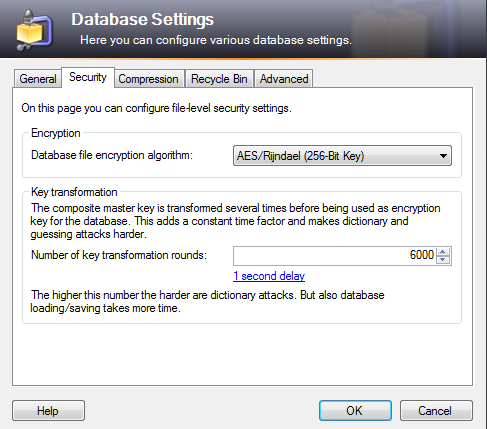
\includegraphics[width=0.7\textwidth]{figures/analysis/keepass_create_security.png}
				\caption{Screenshot of KeePass' security options.}
				\label{fig:keepass_create_security}
			\end{figure}
		
			%\begin{figure}[h!]
			%	\centering
			%	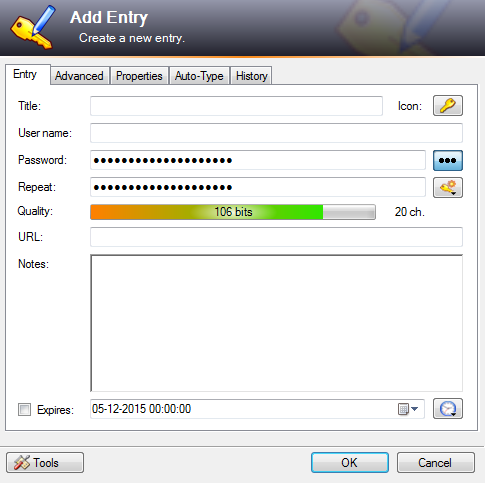
\includegraphics[width=\textwidth]{figures/analysis/keepass_newpassword_main.png}
			%	\caption{.}
			%	\label{fig:}
			%\end{figure}

			\begin{figure}[h!]
				\centering
				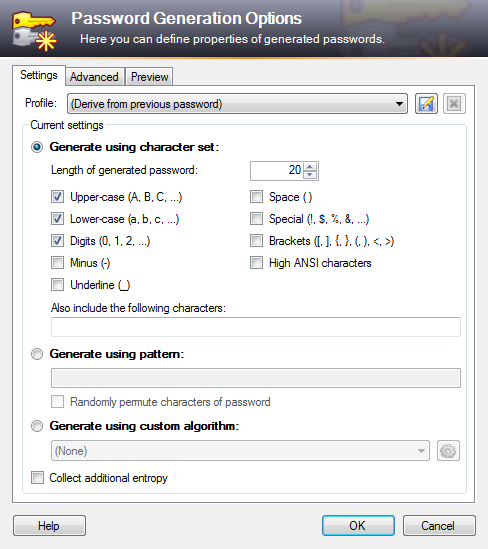
\includegraphics[width=0.7\textwidth]{figures/analysis/keepass_newpassword_passwordgen.png}
				\caption{Screenshot of KeePass' password generator settings.}
				\label{fig:keepass_newpassword_passwordgen}
			\end{figure}

		\subsection*{Rattic}
			Rattic\cite{rattic_frontpage} represents a third type of password manager, and the primary focus of this thesis: A self-hosted password manager, in the so-called private cloud. While at first glance, Rattic seems to be a solution very suited to the problem described earlier, it becomes a far more sketchy solution, upon investigating it closely. Rattic wonderfully describe their solution as:

			\begin{quote}
				\emph{RatticDB is a password management database designed for humans. We have focused on making it able to manage passwords for a team and to make that as easy as possible.}\\\cite{rattic_frontpage}
			\end{quote}

			Since Rattic \emph{is} meant for teams it has multi-user support. Rattic organises passwords and users in groups, and these groups are used for access control. A group is a collection of users, which can access the same passwords. An example of this could be \verb=DevelopmentTeam1= and \verb=DevelopmentTeam2=. Members of team one, can access their own passwords, and members of team two can access theirs, but unless specifically stated, they can not access each others. Additionally it supports tags for their passwords, allowing for even further organisation, for their users allowing quick access to similar passwords, from across different groups.

			However, the fact that Rattic markets itself at teams, rather than individual users is evident by the fact that as per default, you can not create ``private'' passwords, which only a single user can access. To achieve that, you would need to manually create a new group -- per user -- with only said user as member. While this would work, it is very much a work-around of Rattic's default behaviour, for it to work that way.

			From a user experience point of view, Rattic is a rather friendly tool. On figure \ref{fig:rattic_main} on page \pageref{fig:rattic_main}, you see a clean, minimalistic view of available passwords. Granted, this figure is from an Admin's point of view, hence he can access both the \verb=DevelopmentTeam1= and \verb=DevelopmentTeam2= groups, and consequently passwords stored under them.

			\begin{figure}[h!]
				\centering
				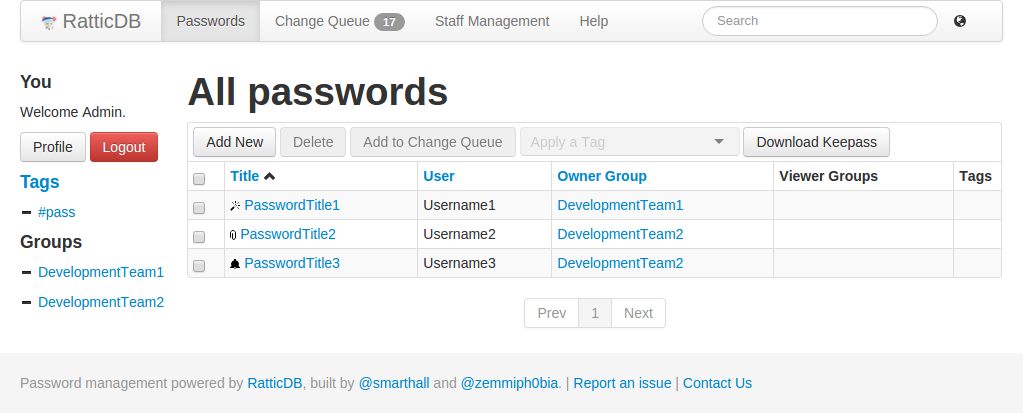
\includegraphics[width=0.95\textwidth]{figures/analysis/rattic_main.png}
				\caption{Rattic's Frontpage of their Web UI.}
				\label{fig:rattic_main}
			\end{figure}

			Adding passwords is just as easy in KeePass, cf. figure \ref{fig:rattic_newpassword_main} on page \pageref{fig:rattic_newpassword_main}. Simply type in the details, select an owner group and submit. While the password generator, cf. figure \ref{fig:rattic_newpassword_passwordgen} on page \pageref{fig:rattic_newpassword_passwordgen}, could stand to have some additional features, it is sufficient for generating strong passwords with high enough entropy. A nifty little feature, is the \verb=Download KeePass= button, which allows a user to download passwords in the KeePass format, making it available for later offline use.

			\begin{figure}[h!]
				\centering
				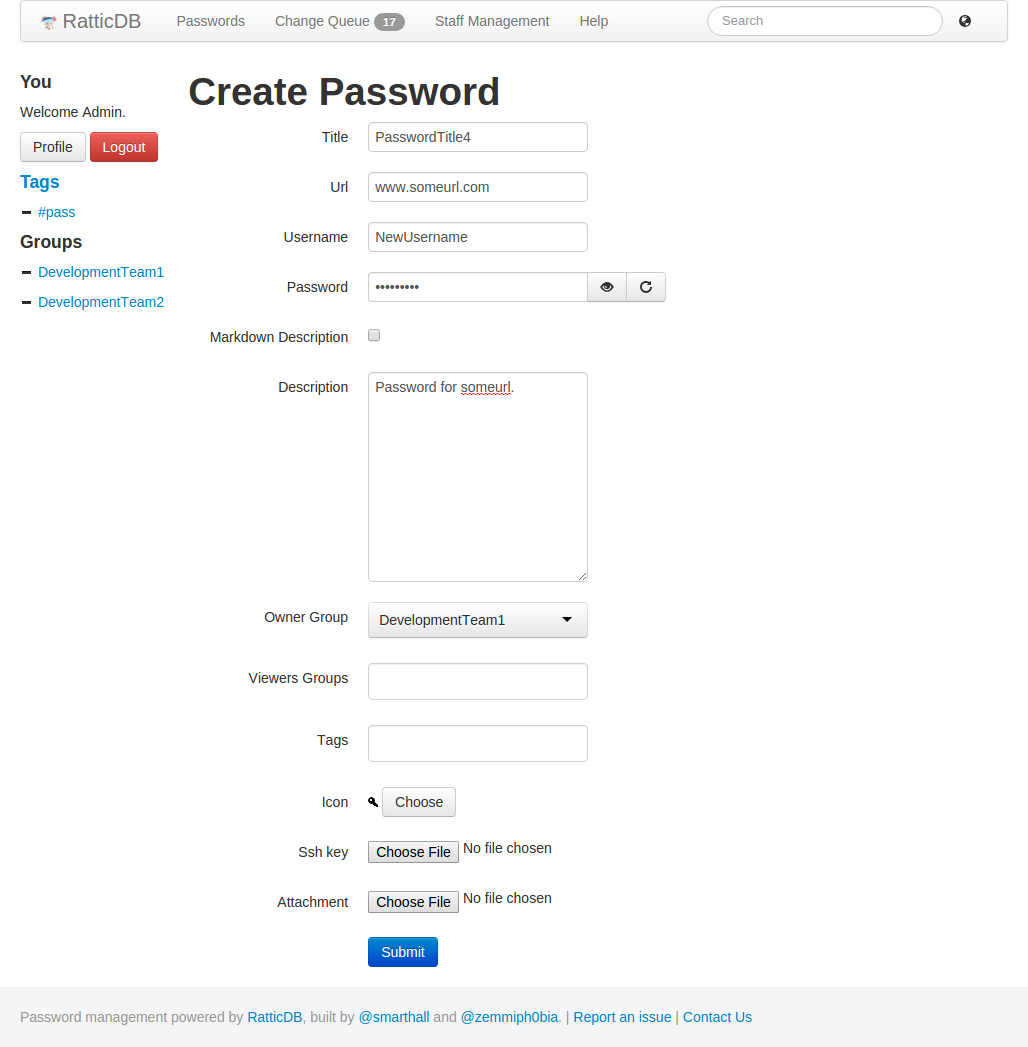
\includegraphics[width=0.95\textwidth]{figures/analysis/rattic_newpassword_main.png}
				\caption{Adding a new password, in Rattic.}
				\label{fig:rattic_newpassword_main}
			\end{figure}

			\begin{figure}[h!]
				\centering
				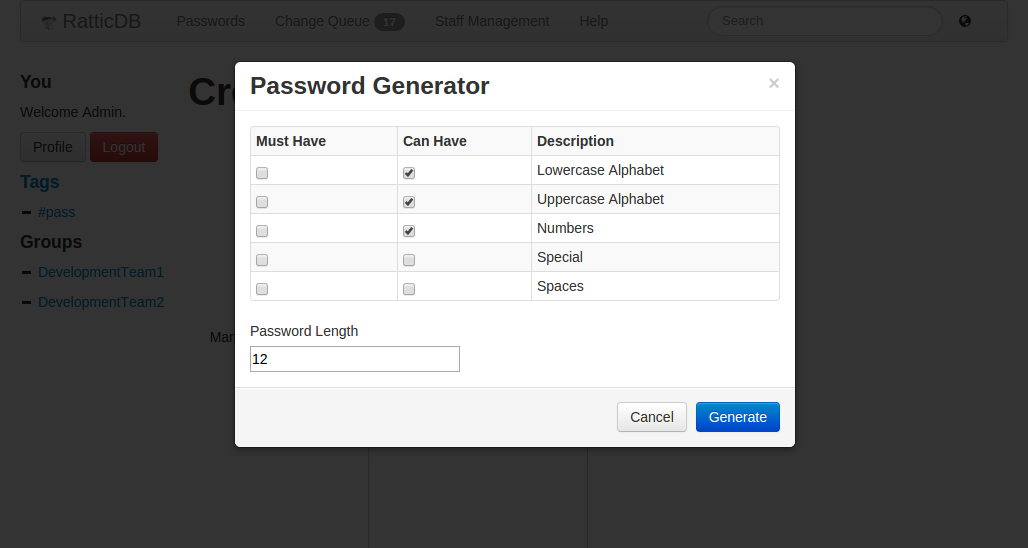
\includegraphics[width=0.95\textwidth]{figures/analysis/rattic_newpassword_passwordgen.png}
				\caption{Generating a password in Rattic.}
				\label{fig:rattic_newpassword_passwordgen}
			\end{figure}

			Having said that, there are some technical concerns, regarding Rattic. Rattic does \emph{not} encrypt passwords stored in the database -- something they are very open about. In \cite{rattic_encryption} they argue heavily for their lack of encryption, due to requiring less code and tests. They do, however, highly recommend storing the database on an encrypted drive, to ensure database protection. However, this \emph{does} mean that a sysadmin can access \emph{all} passwords, should he or she have the encryption key for the drive. Due to this, the deployment of Rattic is fairly complex, as they admit themselves. 

			Rattic is developed in Python, using the Django framework and tested on the Apache server.

		\subsection*{Encryptr}
			Bordering between the type of LastPass and Rattic, Enryptr \cite{encryptr} relies on the Crypton\cite{crypton} backend\cite{encryptr_backend}, available hosted at SpiderOak\cite{crypton_spideroak}. Per default, Encryptr \emph{only} supports hosting passwords at the Crypton backend, hosted at SpiderOak. However, it \emph{is} possible to run this in the private cloud, with your own Crypton backend. \emph{But} it requires manually editing source files\cite{encryptr_selfhost}, which makes the setup a pain. So not only would you have to set up Crypton, and its requirements, you would have to download the source of the apps, change the specified line of code, compile and \emph{then} you could use it. Because of this technical aspect, usability is virtually zero, as you would need to be fairly confident behind a keyboard, to successfully set this up.

			Having said that, the UI of Encryptr is \emph{very} minimalistic and sleek, which both is a good and a bad thing. As seen on figure \ref{fig:encryptr_main} on page \pageref{fig:encryptr_main}, all passwords are stored in a \emph{single} list: There is \emph{no} organisation, other than labels. Granted, they do support searching, but somehow that still makes it very confusing, if more than a handful of passwords or secrets are stored, and since Encryptr not only supports storing passwords, but also credit card information and general secrets, this could be achieved fairly quickly.

			Adding a passwords shows something disturbing: Lack of a decent password generator, cf. figure \ref{fig:encryptr_newpassword} on page \pageref{fig:encryptr_newpassword}. Once the form for adding a new password is opened, a password is generated as per some default behaviour. There is no customising entropy of the password, or even something as simple as the length.

			\begin{figure}[h!]
				\centering
				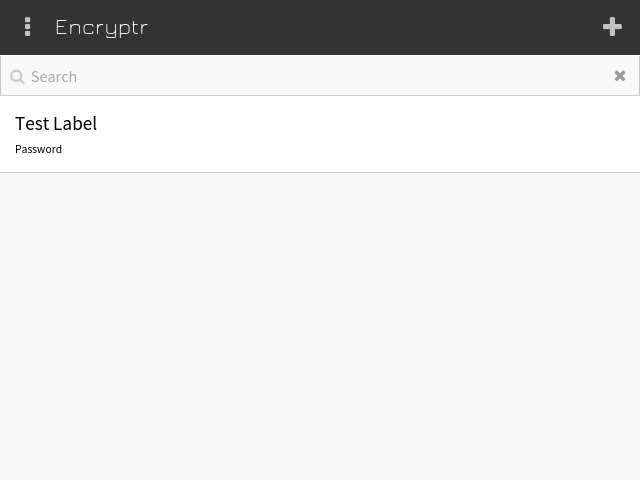
\includegraphics[width=0.75\textwidth]{figures/analysis/encryptr_main.png}
				\caption{Encryptr's main view.}
				\label{fig:encryptr_main}
			\end{figure}


			\begin{figure}[h!]
				\centering
				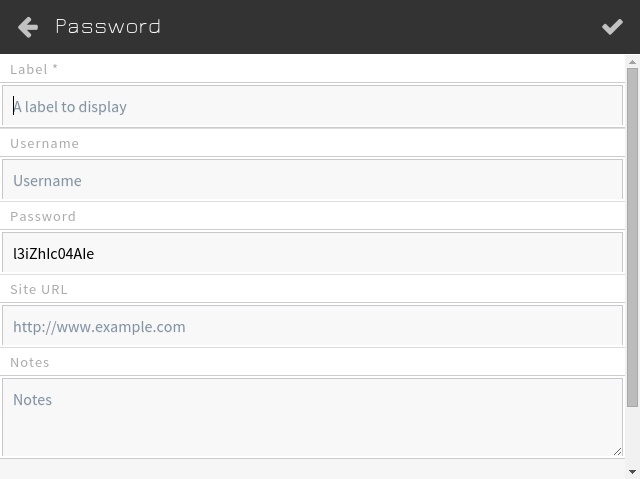
\includegraphics[width=0.75\textwidth]{figures/analysis/encryptr_newpassword_main.png}
				\caption{Adding a new password in Encryptr.}
				\label{fig:encryptr_newpassword}
			\end{figure}

			On the technical side, Crypton -- the backend -- is actually fairly interesting. Using their own definition of zero-knowledge, the developers created a complete framework for securely transferring and storing data at a remote machine\cite{crypton_paper}. They claim, that it is impossible to obtain the unencrypted data on their servers, without actually getting hold of the users private encryption key. The Crypton backend is open source, and available at \cite{crypton_git}. What powers Crypton, cryptographically speaking, is AES-256.

		\subsection*{Vault}
			Vault\emph{(ZOHO)}\cite{vault_zoho} is another piece of software, that requires you to submit your data to their servers. Where this tool differs from LastPass and Encryptr, is that it is \emph{clearly} aimed at enterprise customers, which is clearly evident based on their features, such as LDAP integration.

			Vault organises the passwords in so called Chambers. Each password \emph{can} be added to one or more chambers, but is not necessary. Seen on figure \ref{fig:vaultzoho_main_secrets} on page \pageref{fig:vaultzoho_main_secrets} we see how it lists all available passwords, in a single list. Using this main list quickly becomes very confusing. Looking at the Chambers list, which is found on figure \ref{fig:vaultzoho_main_chambers} on page \pageref{fig:vaultzoho_main_chambers}, the same pattern arises again. A large list, showing only the important information -- the passwords -- in the smallest part of the UI. All in all, performing simple tasks is very clunky.

			As with Encryptr, password generation lacks a lot. A password can be generated -- and re-generated -- but it happens after some under-the-hood-behaviour, which the user can not choose to customise.


			\begin{figure}[htbp]
				\centering
				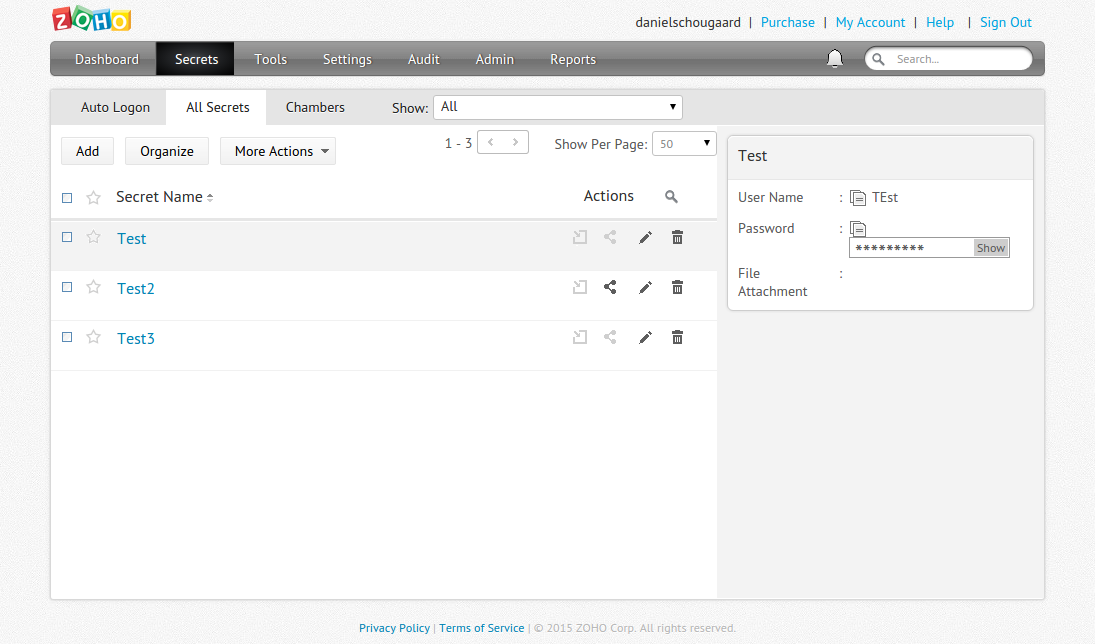
\includegraphics[width=0.95\textwidth]{figures/analysis/vaultzoho_main_secrets.png}
				\caption{Listing all stored secrets in Vault \emph{(ZOHO)}.}
				\label{fig:vaultzoho_main_secrets}
			\end{figure}

			\begin{figure}[htbp]
				\centering
				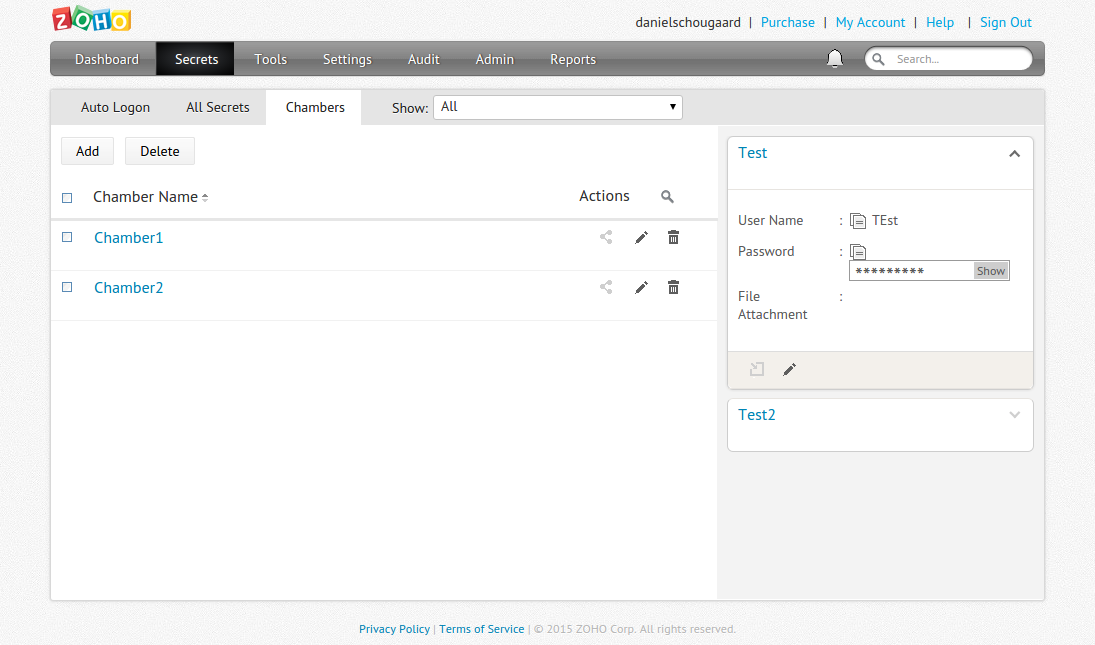
\includegraphics[width=0.95\textwidth]{figures/analysis/vaultzoho_main_chambers.png}
				\caption{Listing Chambers stored in Vault \emph{(ZOHO)}.}
				\label{fig:vaultzoho_main_chambers}
			\end{figure}


			Under the hood, Zoho uses a combination of RSA and AES. To enable sharing, a common AES encryption key is retrieved using RSA keypairs, from the admin, and users involved in sharing\cite{vault_zoho_encryption}.

		\subsection*{TeamPasswordManager}
			TeamPasswordManager\cite{teampasswordmanager_frontpage} \emph{(henceforth referred to as TPM)} is a tool that is fairly similar to Rattic. However, where it differs is the less minimalistic UI. TPM organises passwords in ``Projects'', which is a great indicator that this tool is in fact intended to be used with enterprise in mind. TMP is able to be self-hosted and is platform independent, requiring Apache, PHP and MySQL, which is a great asset.

			Turning to the user experience, the frontpage that the user is presented with, as seen in figure \ref{fig:teampasswordmanager_main} on page \pageref{fig:teampasswordmanager_main}, is a clunky list of all available passwords. For organisational value, groups as ``Favorite'' and ``Recent'' are also available, filtering the available passwords into more manageable lists. But once again, this very clunky and large UI is used, much like in Vault.

			TeamPasswordManager aims itself at -- as the name implies -- teams, much like Rattic. This choice, is very apparent in the work flow. For instance, a password is tied to a ``project", instead of a user. Where TPM excels, is the fact that a project can contain sub-projects, which in return can contain sub-projects, and so forth. This creates a tree-like structure, much like that of KeePass, which can be seen on figure \ref{fig:teampasswordmanager_tree} on page \pageref{fig:teampasswordmanager_tree}.


			\begin{figure}[htbp]
				\centering
				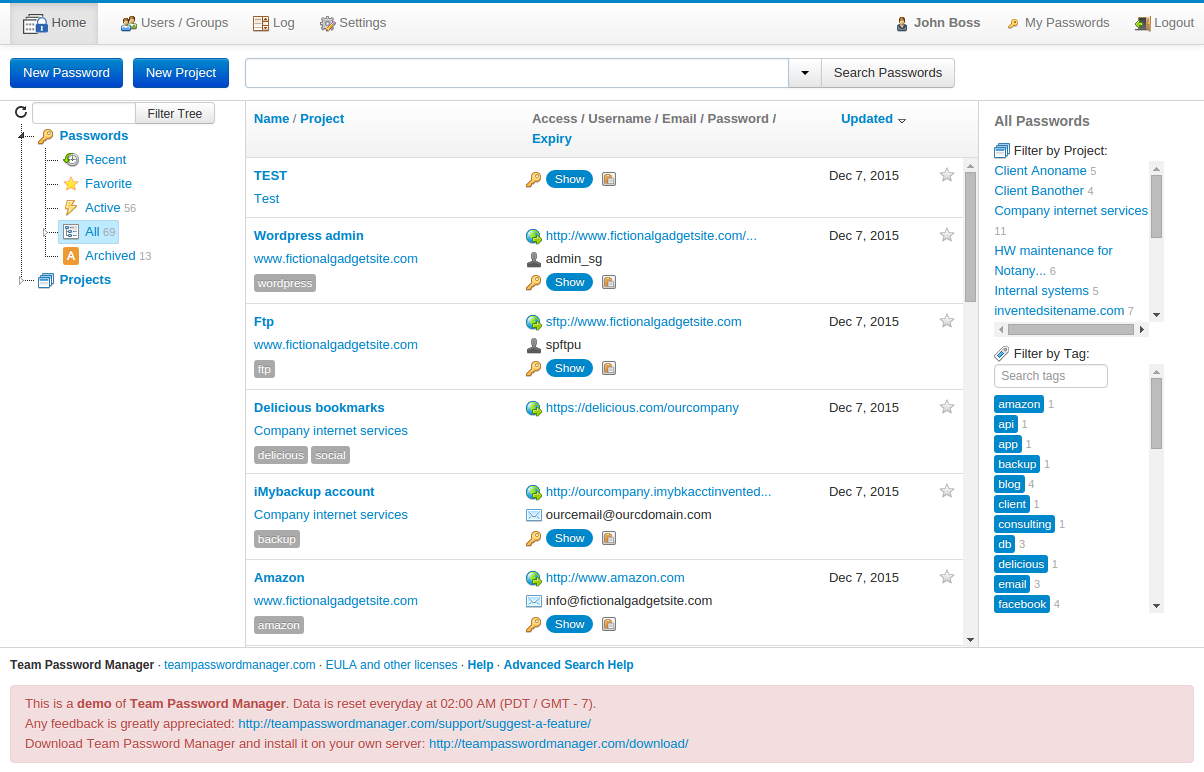
\includegraphics[width=0.95\textwidth]{figures/analysis/teampasswordmanager_main.png}
				\caption{Front page of TeamPasswordManager's web interface.}
				\label{fig:teampasswordmanager_main}
			\end{figure}

			\begin{figure}[htbp]
				\centering
				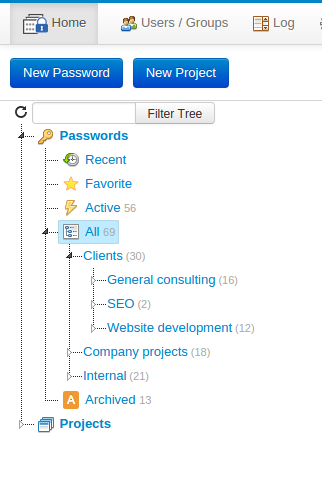
\includegraphics[width=0.35\textwidth]{figures/analysis/teampasswordmanager_tree.png}
				\caption{The tree-like organisational structure of TeamPasswordManager.}
				\label{fig:teampasswordmanager_tree}
			\end{figure}

			Encryption wise, TPM uses the same basic algorithm we've seen over and over again: AES-256. TPM also uses bcrypt as their chosen key derivation function, to make it as difficult for a potential attacker to brute force password hashes. Using Google's Authenticator, it supports two-factor authentication.

			While this software could essentially suffice, in order to meet the requirements, it would be lacking heavily in the user experience department. Additionally, it provides features and information, which would only be of use to super-users, and enterprise users, and might very well scare off regular users.

		\subsection*{Passwordstate}
			Passwordstate from ClickStudios\cite{passwordstate} is a solution some-what similar to both TeamPasswordManager and Vault \emph{(Zoho)}. There is not a seconds doubt, that this is a solution aimed at enterprise users, as they state themselves. This is also evident by the feature set, they have: Sporting not only active directory support, they also have built-in options for High Availability and \emph{several} options for two-factor authentication, amongst others. Passwordstate is self-hostable, but requires a windows platform and the IIS server \cite{passwordstate_requirements}.

			Inspecting the user experience, reveals that Passwordstate is a fresh breeze. This solutions actually manages to give the most important information, the most screen-space. On figure \ref{fig:passwordstate_main} on page \pageref{fig:passwordstate_main}, we see how password state allows for the same tree-like structure, that we've seen before. This creates excellent organisational options, for the users. On the frontpage the user is presented with his or hers favourite passwords list, and recently accessed passwords. Alas, here is where Passwordstate falls short. Instead of keeping a minimalistic UI, the user is presented with information, only interesting to enterprise users, or super-users. A host list, is with a high probability useless for the majority of regular users, as well as the little graph that shows password statistics, as seen on figure \ref{fig:passwordstate_graph} on page \pageref{fig:passwordstate_graph}. This particular graph, presented at this particular place, seems very much to be a graph for the sake of a graph. 

			Additionally, accessing passwords is not straight forward: Again, Passwordstate presents the user with a \emph{lot} of enterprise options, which is far from beneficial for a regular user. The available options can be seen on figure \ref{fig:passwordstate_getpassword} on page \pageref{fig:passwordstate_getpassword}. Taken all of these things into consideration, Passwordstate is an excellent password manager for enterprises, already running Windows as their server software. However, for regular home users, the software is simply \emph{far} too complex.

			Passwordstate has the options to completely customise the rules, that a password is generated by, much like KeePass. On figure \ref{fig:passwordstate_newpassword_passwordgen} on page \pageref{fig:passwordstate_newpassword_passwordgen} you see the \emph{extensive} options, enabling the user to customise the password to their needs.

			\begin{figure}[htbp]
				\centering
				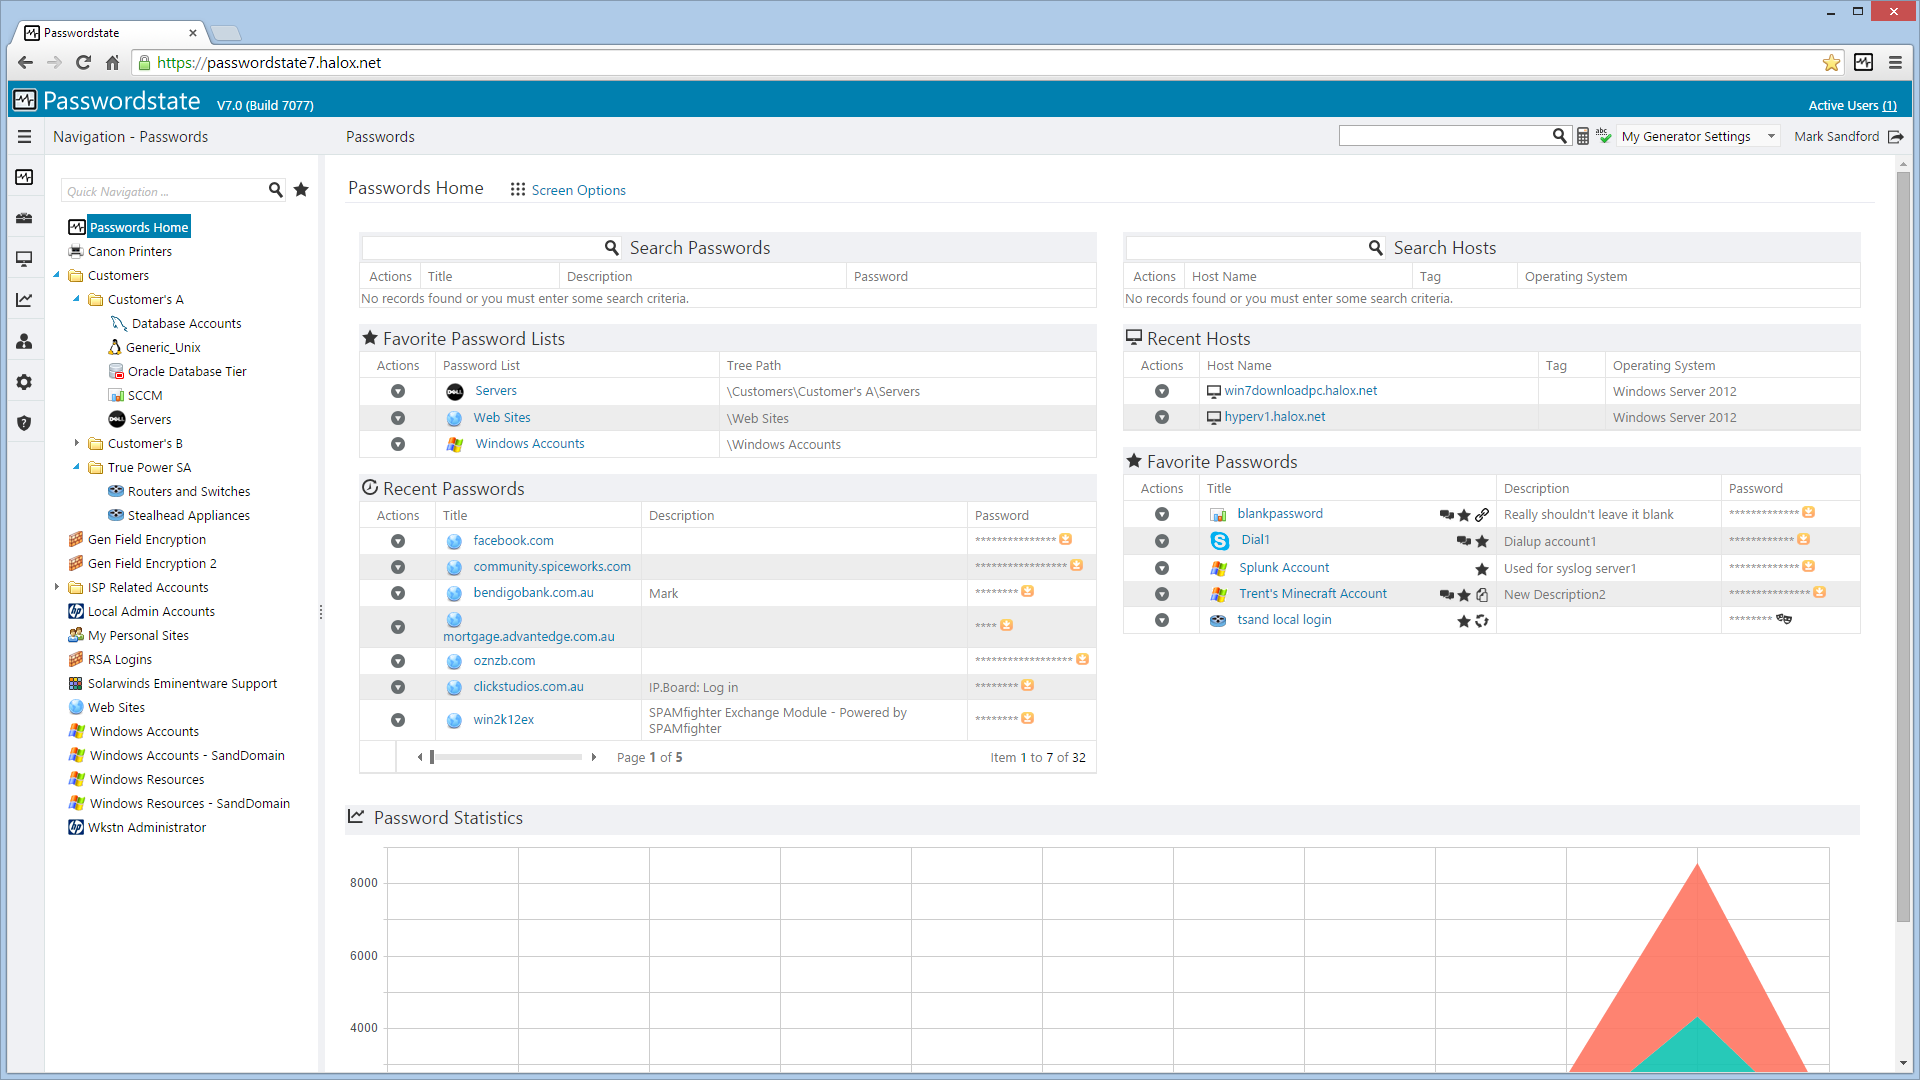
\includegraphics[width=0.95\textwidth]{figures/analysis/passwordstate_main.png}
				\caption{Frontpage of the PasswordState website. \figsrc{fig:passwordstate_main} }
				\label{fig:passwordstate_main}
			\end{figure}

			\begin{figure}[htbp]
				\centering
				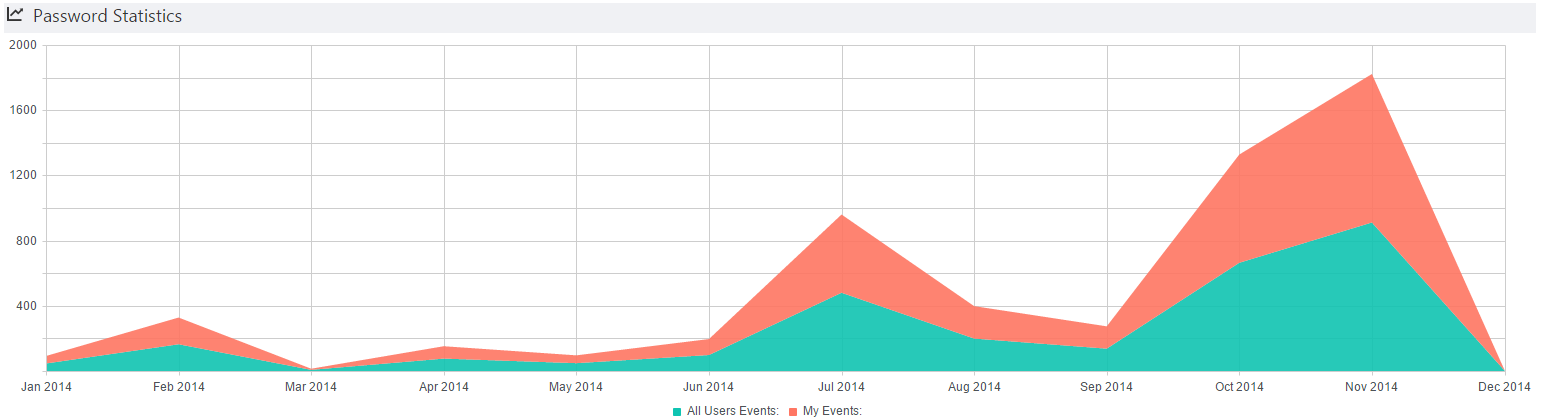
\includegraphics[width=0.95\textwidth]{figures/analysis/passwordstate_graph.png}
				\caption{Password statistics graph, in PasswordState. \figsrc{fig:passwordstate_getpassword}}
				\label{fig:passwordstate_graph}
			\end{figure}

			\begin{figure}[htbp]
				\centering
				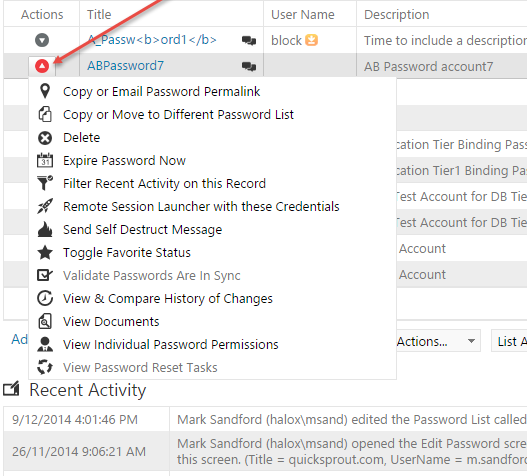
\includegraphics[width=0.7\textwidth]{figures/analysis/passwordstate_getpassword.png}
				\caption{Retrieving a password in PasswordState. \figsrc{fig:passwordstate_graph}}
				\label{fig:passwordstate_getpassword}
			\end{figure}

			\begin{figure}[htbp]
				\centering
				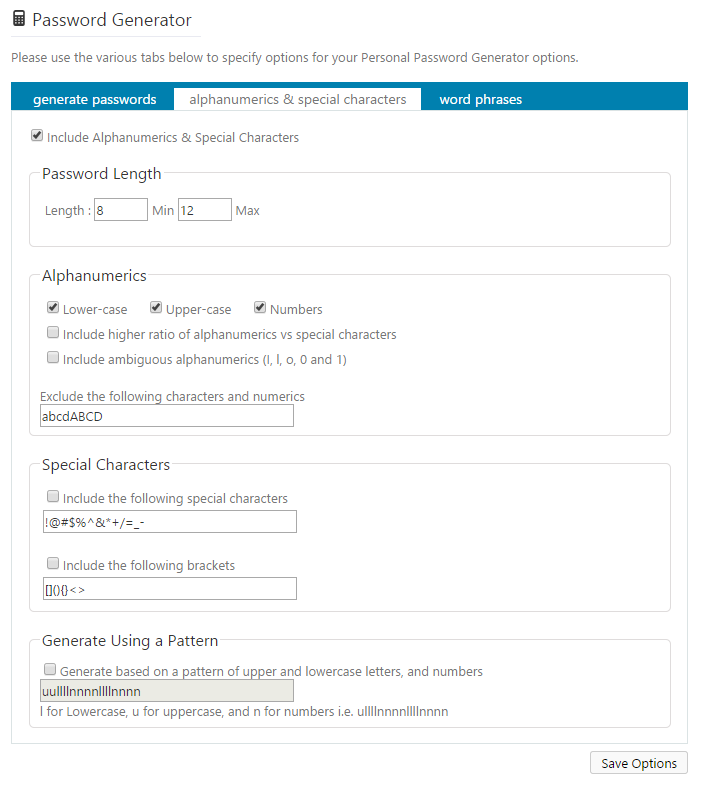
\includegraphics[width=0.95\textwidth]{figures/analysis/passwordstate_newpassword_passwordgen.png}
				\caption{Generating a new, secure, password in Passwordstate. \figsrc{fig:passwordstate_newpassword_passwordgen}}
				\label{fig:passwordstate_newpassword_passwordgen}
			\end{figure}

			Looking at the technical side, Passwordstate encrypts all passwords using AES-256\cite{passwordstate_security}, which seems to be the standard. Additionally, all sensitive information is salted. Passwordstate protects their sourcecode by the use of:
			\begin{quote}
				\emph{... precompiled ASP.NET pages and obfuscated .NET Assemblies. No longer can web or database administrators gain access to data they are not authorised to view. }\cite{passwordstate_security}
			\end{quote}

			Unfortunately, the limited number of platforms Passwordstate can run on, is a \emph{huge} drawback.

		\subsection*{SimpleSafe}
			SimpleSafe\cite{simplesafe} is another take on the self-hosted team password manager solution, which seems to be the predominant solution available. Unfortunately SimpleSafe's documentation is lacking heavily, but based on their available demo, it appears that all users have access to all passwords. This results in that a single user can not have a private password, for their use only.

			While it appears they have whole-heartedly embraced the idea of a minimalistic design, they've done so at the expense of user experience. The main view is a rather large but accessible list, with customizable attributes. On figure \ref{fig:simplesafe_main} on page \pageref{fig:simplesafe_main} the list is shown. The user can chose to organise passwords \emph{(or custom entries)} into groups. Groups are accessed through a menu, which is auto hidden. The expanded menu is shown on figure \ref{fig:simplesafe_menu} on page \pageref{fig:simplesafe_main}. Unfortunately, changing between groups takes a \emph{long} time. This causes a horrible experience for the user. Generally, the developers of SimpleSafe have been very generous with the animations, as pretty much all actions in the UI invokes some kind of animation. The delays because of this, adds to the overall sluggish feel of the system.

			\begin{figure}[htbp]
				\centering
				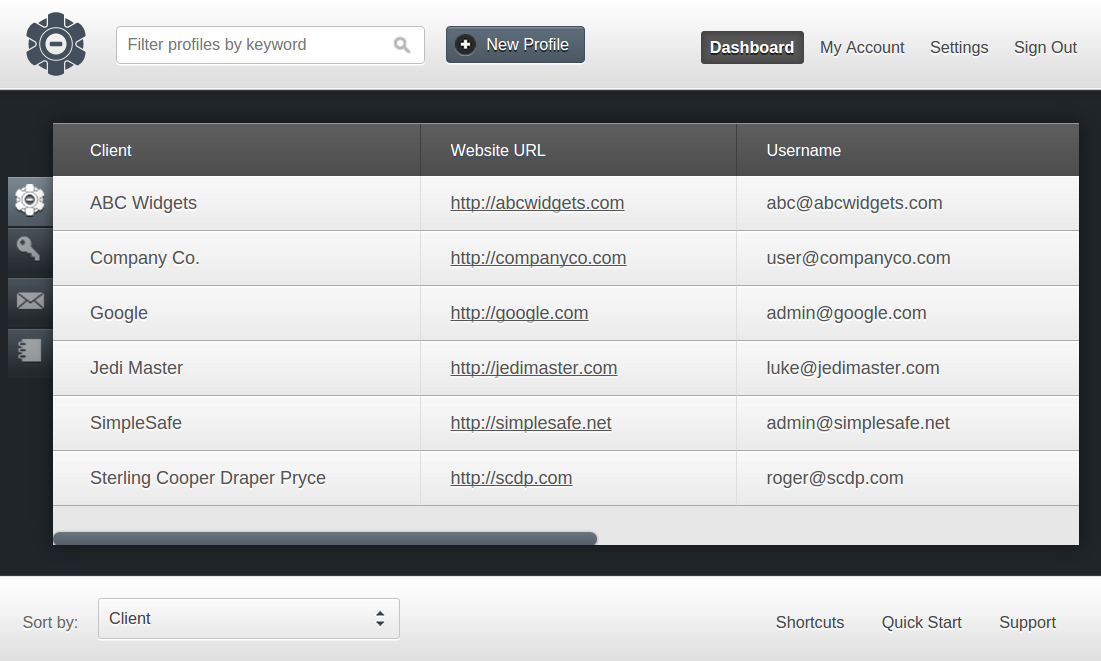
\includegraphics[width=0.95\textwidth]{figures/analysis/simplesafe_main.png}
				\caption{Homepage of SimpleSafe}
				\label{fig:simplesafe_main}
			\end{figure}

			\begin{figure}[htbp]
				\centering
				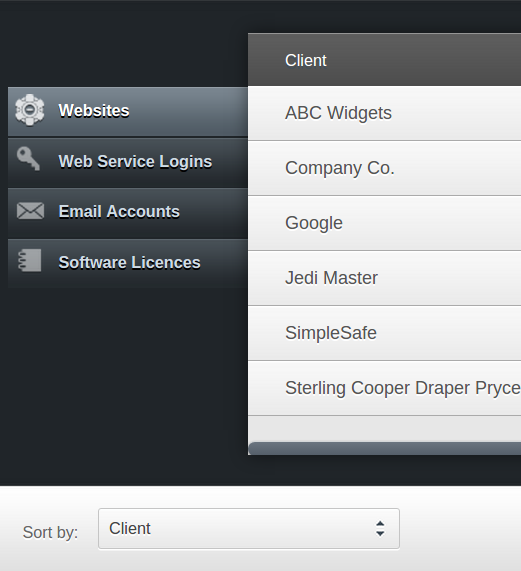
\includegraphics[width=0.70\textwidth]{figures/analysis/simplesafe_groups.png}
				\caption{Menu for changing groups in SimpleSafe.}
				\label{fig:simplesafe_menu}
			\end{figure}

			Security wise, it is \emph{very} difficult to inspect SimpleSafe, due to their own lack of description. The only available information regarding security or encryption is the following quote.
			\begin{quote}
				\emph{SimpleSafe utilises a 256 bit encryption method. Each password has a unique private salt along with a master salt stored separately to the database. Only encrypted passwords are stored within the database.}\cite{simplesafe_faq}
			\end{quote}

			All in all SimpleSafe is a \emph{fairly} sketchy solution. One thing that is pretty neat, is the ability for a user to customise the fields in the different groups. For instance, they allow you to store SSH keys, in a particular field type. This lets the user separate things that require keys / certs, from traditional username/password logins.

		\subsection*{PassWork}
			PassWork\cite{passwork} is yet another take, on the same type of solution as SimpleSafe, Rattic, TeamPasswordManager, and Passwordstate. PassWork is available as both a remote and a self-hosted solution, both of which comes with a price tag. 

			PassWork organises passwords in groups, which in return can contain sub-groups -- or folders as the icon resembles. Each group has a list of users, currently allowed to access passwords in said group. As figure \ref{fig:passwork_adduser} on page \pageref{fig:passwork_adduser} shows, users can be added to groups, with permissions ``Full Access'', ``Edit'', and ``Read''. While differentiating between ``Edit'' and ``Full Access'' might be difficult, the option of setting permissions \emph{that} easily, when adding a user, is surprisingly a very good feature. Per default a group called a ``My passwords'' group is created, in which the user can place private passwords. 

			\begin{figure}[htbp]
				\centering
				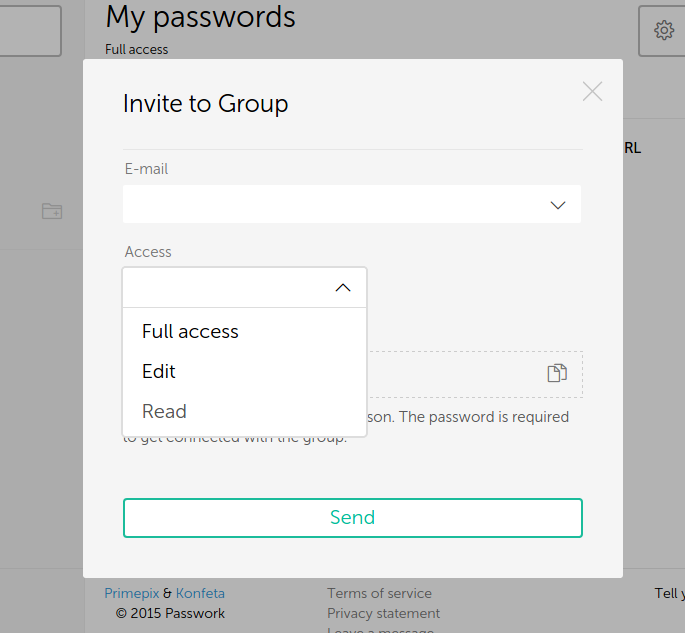
\includegraphics[width=0.95\textwidth]{figures/analysis/passwork_adduser_cropped.png}
				\caption{Permissions available, when adding users to a group.}
				\label{fig:passwork_adduser}
			\end{figure}

			PassWork is another example of developers not describing and documenting their soltion properly. Something as simple as figuring out which platform it supports, prior to purchasing is not possible. Additionally it is impossible to completely determine their encryption scheme, but they use ``256-bit passwords'' and RSA keypairs for sharing passwords. 

			Their less than completely transparency when it comes to choice of encryption algorithm not to mention the hefty price-tag, should one wish to self-host it. Additionally, they completely omit to inform which platform(s) the self-hosted version is able to be run on.

		\subsection*{SimpleVault}
			Taking a bit of a different route from other solutions, SimpleVault\cite{simplevault} chooses to encrypt each individual password, with a different ``passphrase''. Based on their user experience, it would seem that SimpleVault is a proof of concept, more than a release software. Something as simple as headers for the table containing the main information is missing, as seen on figure \ref{fig:simplevault_main} on page \pageref{fig:simplevault_main}.

			Adding a password, on figure \ref{fig:simplevault_addpassword}, shows the same lack of attention to the user experience, having two fields completely undescribed. One thing that SimpleVault \emph{does} get right in this context, is the option to generate passwords. Three buttons exists for generating passwords, with increasinly ``rare'' symbols. While options for passwords of specific length lacks, it seems to -- per default -- generate password of suitable length. 

			Retrieving a password, on figure \ref{fig:simplevault_getpassword}, requires the user to type in the passphrase. The choice of this per-password passphrase, will undoubtedly only result in the user using the same password over and over again. However, this choice \emph{does} allow for the system to be used by multiple users, each just using their own master passphrase for all of their passwords.

			\begin{figure}[htbp]
				\centering
				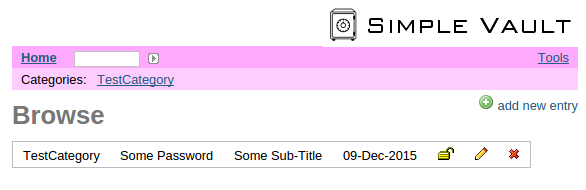
\includegraphics[width=0.95\textwidth]{figures/analysis/simplevault_main.png}
				\caption{Frontpage of SimpleVault.}
				\label{fig:simplevault_main}
			\end{figure}

			\begin{figure}[htbp]
				\centering
				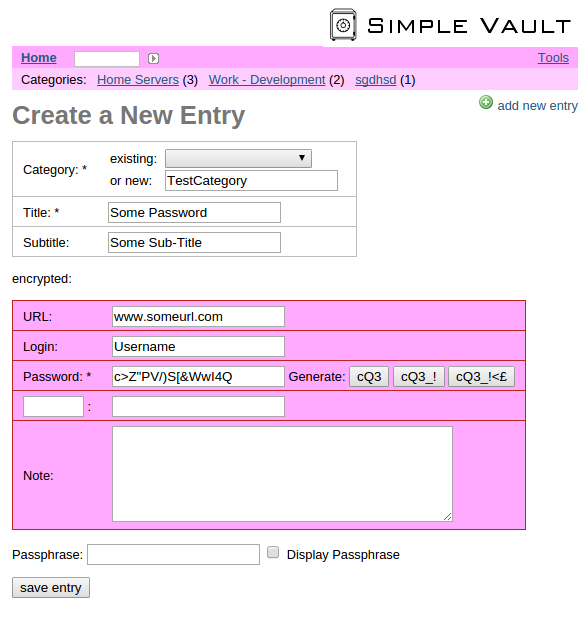
\includegraphics[width=0.95\textwidth]{figures/analysis/simplevault_newpassword.png}
				\caption{Adding a password to be stored in SimpleVault.}
				\label{fig:simplevault_addpassword}
			\end{figure}

			\begin{figure}[htbp]
				\centering
				\begin{subfigure}{\textwidth}
					\centering
					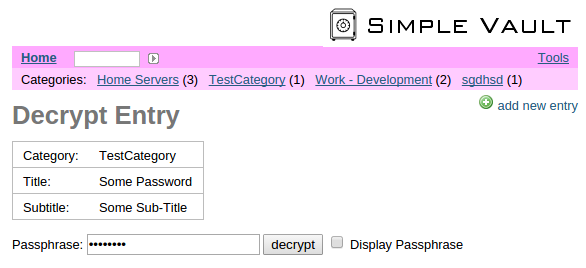
\includegraphics[width=0.95\textwidth]{figures/analysis/simplevault_getpassword.png}
					\caption{Typing passphrase, in order to decrypt stored password.}
					\label{fig:simplevault_getpassword_type}
				\end{subfigure}%
				
				\begin{subfigure}{\textwidth}
					\centering
					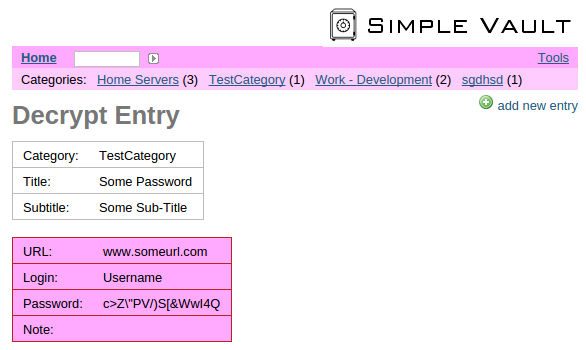
\includegraphics[width=0.95\textwidth]{figures/analysis/simplevault_getpassword_decrypted.png}
					\caption{Decrypted password shown in SimpleVault}
					\label{fig:simplevault_getpassword_decrypted}
				\end{subfigure}
				
				\caption{Process of retrieving a password in SimpleVault.}
				\label{fig:simplevault_getpassword}
			\end{figure}


			Security wise SimpleVault is quite horrible. With what can be taken from the quite poor description of the security of the system, the encrypted data is actally \emph{stored in clear text} on the remote machine, at some point or other. When adding a new entry, the password is sent in \emph{clear text} to the server, which then encrypts it. The developer argues that this is fine, as long as only HTTPS is used, for communicating with the server, but regardless of which protocol is used the password is \emph{still} stored in clear text. Additionally, SimpleVault does \emph{not} use a database system, but stores all contents in a \verb=.txt= file. 

			All in all, SimpleVault is probably a tool \emph{no one} should use. No matter their problem at hand.

		\subsection*{RoboForm}
			RoboForm\cite{roboform} is somewhat a hybrid between the likes of KeePass and LastPass. While at heart, RoboForm is a locally stored password manager, it only exists as a browser extension. Since it only exist as a browser plugin, features such as form auto fill etc. are of course in their repertoire. However, from a ux point of view, the plugin stands out quite a bit from the browser. While this is a relatively small complaint, the usage of design guidelines from both Apple and Google, has helped create platform standards for how apps are supposed look, so the user never feels lost. Additionally, they offer ``RoboForm Everywhere'' cloud synchronisation of the encrypted file. This does however, entail trusting them with safe-keeping the encrypted file.

			Using RoboForm on a single device, renders it as a tool very similar to KeePass, albeit with ``better'' browser integration. Using RoboForm Everywhere results in the same downsides and threats, as previously explained.

		\subsection*{Vaultier}
			At a first glance, Vaultier\cite{vaultier} seems to be everything one would want in the private cloud: Its self-hosted, the latency for actions in the user interface is close to none, and the design of the frontpage is clean. Even installing it comes easy, as it is shipped with a self-contained docker image. However, digging deeper, short comings starts to arise.

			Their choice of organisation is confusing at first. At first you have a workspace, in which vaults are placed. Inside of these vaults, cards are placed. Inside of these cards, passwords are placed. The real problem comes when trying to add items into the vaults. Inside a single vault, you can at most have six cards shown at a time, on a standard 1080p monitor, cf. \ref{fig:vaultier_cards} on page \pageref{fig:vaultier_cards}. The same issue applies when looking at passwords: At most two passwords can be displayed on screen, at a time, cf \ref{fig:vaultier_passwords} on page \pageref{fig:vaultier_passwords}.

			Since RightClick has chosen to have the git repository's history publicly shown, it can be determined the last time it was maintained. That was the 17th of April, 2015\cite{vaultier_history}. It would seem that the project has been abandoned and is dead. As such, it is not a stretch to assume that the project will not be kept up to date, in regards to deprecated dependencies or new-found bugs and security holes.



			\begin{figure}[htbp]
				\centering
				\includegraphics[width=0.95\textwidth]{figures/analysis/vaultier_passwords_lined.png}
				\caption{List of available passwords inside a card, in Vaultier. The dotted line represents the bottom of the browser window, maximized on a 1080p screen.}
				\label{fig:vaultier_passwords}
			\end{figure}
			\begin{figure}[htbp]
				\centering
				\includegraphics[width=0.95\textwidth]{figures/analysis/vaultier_cards_lined.png}
				\caption{List of available cards inside a vault, in Vaultier. The dotted line represents the bottom of the browser window, maximized on a 1080p screen.}
				\label{fig:vaultier_cards}
			\end{figure}

		\subsection*{TeamPass}
			From a technical point of view TeamPass might be considered a decent option. Ensuring platform agnosticism due to being implemented in PHP, it only requires an Apache server and MySQL server to run. 

			Boasting of having an API to ``permit an access to Teampass Items from a third party application'', they a disturbing lack of security concerns. Examining their call for retrieving the password for a specific site, some very odd behaviour is present. First and foremost, what surely should have been a RESTful API, is implemented \emph{only} using the \verb=GET= HTTP method. Secondly, their API states that a user's password is sent \emph{in} the URL, as part of the \verb=GET= call. This is a huge blunder, from the developer's part. 

			Additionally, based on the description of their API, it would appear as if the password is decrypted server-side. This goes against the requirements previously specified.
			\begin{verbatim}
				<url to teampass>/api/index.php/auth/<PROTOCOL>/<URL>_
				/<user login>/<user password>?apikey=<VALID API KEY>
			\end{verbatim}
			Where they describe the parameters as
			\begin{verbatim}
				< PROTOCOL > : is the protocol used for the URL (example: http	https	ftp	…)
				< URL > : is the URL without the protocol (example:_
				 http://www.teampass.net becomes www.teampass.net)
				< user login > : user’s login
				< user password > : user clear password
				< VALID API KEY > : api key for access validation
			\end{verbatim}

		\subsection{Final Comparisons}
			% Table color shortcuts
			\newcommand{\red}[1]{\cellcolor{red!75}#1}
			\newcommand{\green}[1]{\cellcolor{green!75}#1}
			\newcommand{\grey}[1]{\cellcolor{gray!75}#1}
			\newcommand{\yellow}[1]{\cellcolor{yellow!75}#1}
			\newcommand{\white}[1]{\cellcolor{white!75}#1}


			While the previous sections covered an in-depth look at the various solutions, it might seem a little overwhelming. Here, the information will be condensed into tables, for a better picture of the differences between the various solutions.

			First and foremost, on table \ref{tbl:web_based} on page \pageref{tbl:web_based}, a clear cut distinction is seen: The solutions that are \emph{able} to be run in the private cloud, and those who isn't. Focussing only on those which actually \emph{can} exist in the private cloud, on table \ref{tbl:passwords} on page \pageref{tbl:passwords} their default approach to passwords are compared. While all of the systems support multiple users in \emph{some} way, they all pretty much share the same sigh on personal passwords: They should not exist. This is primarily a result of nearly all of these being marketed towards teams. For almost all of the solutions, the same approach to solving this shortcoming is the same: Create a new \emph{personal} group for each individual user, in which personal passwords can be stored. Unfortunately, this \emph{must} be considered a workaround, with the exception of PassWork, in which this group is created automatically. 

			Looking at the more technical aspect of the comparison, on table \ref{tbl:agnostic} on page \pageref{tbl:agnostic} a comparison of their agnosticism is made. Most of the solutions are able to be run on multiple platforms, due to being implemented in PHP. Hence, they only require an Apache \emph{(or nginx)} server to be run. Fortunately, both of these have versions for all major operating systems. Unfortunately, there is only one solution that actually has options for various database solutions. \emph{But} the developers note, that this is done at the user's risk, since they're not tested as rigorously.

			By comparing these three tables, it is unfortunately seen that there isn't \emph{one} completely fulfilling the requirements earlier specified.



			\begin{table}
				\begin{minipage}{1.0\textwidth}
					\begin{tabular}{| r | l | l |}
						\hline
						Name 						& Web Based 			& Self-Hostable 		\\
						\hline
						LastPass 					& \green{Yes}			& \red{No} 				\\
						\hline
						KeePass 					& \red{No} 				& \grey{N/A} 			\\
						\hline
						Rattic 						& \green{Yes} 			& \green{Yes}  			\\
						\hline
						Encryptr 					& \red{No} 				& \yellow{Yes} \footnote{Requires editing source files and running own Crypton backend.} 			\\
						\hline
						Passwordstate 				& \green{Yes} 			& \green{Yes}  			\\
						\hline
						Vault \emph{(Zoho)} 		& \green{Yes} 			& \red{No} 				\\
						\hline
						TeamPasswordManager 		& \green{Yes} 			& \green{Yes}  			\\
						\hline
						Simple Safe 				& \green{Yes} 			& \green{Yes}  			\\
						\hline
						Passwork 					& \green{Yes} 			& \green{Yes}  			\\
						\hline
						SimpleVault 				& \green{Yes} 			& \green{Yes}  			\\
						\hline
						RoboForm 					& \red{No} 				& \grey{N/A} 			\\
						\hline
						TeamPass 					& \green{Yes} 			& \green{Yes}  			\\
						\hline
						Vaultier 					& \green{Yes} 			& \green{Yes}  			\\
						\hline
					\end{tabular}
				\end{minipage}
				\caption{Comparison of access method and ownership model, of the available solutions.}
				\label{tbl:web_based}
			\end{table}


			%% Footnotes for Table tbl:agnostic
			\newarray\tblPasswordsFN
			\tblPasswordsFN(1)={Through password grouping.\label{fn:passwords:group}}
			\tblPasswordsFN(2)={Through a commonly used master passphrase, acting as a work-around.\label{fn:passwords:common_masterpassphrase}}
			\tblPasswordsFN(3)={By each user, using their own unique passphrase for encrypting their personal passwords.\label{fn:passwords:unique_masterpassphrase}}
			\begin{table}
				\begin{minipage}{1.0\linewidth}
					\begin{tabular}{ | p{0.30\textwidth} | p{0.25\textwidth} | p{0.15\textwidth} | p{0.15\textwidth} | }
						\hline
						\textbf{Name}  		& \textbf{Supports Multiple Users} 			& \textbf{Personal Passwords} 					& \textbf{Password Sharing} \\
						\hline
						Rattic 				& \green{Yes} 								& \yellow{Yes}\footnote{\tblPasswordsFN(1)}		& \green{Yes} 				\\
						\hline
						Passwordstate 		& \green{Yes} 								& \yellow{Yes}\footref{fn:passwords:group}		& \green{Yes}				\\
						\hline
						TeamPasswordManager & \green{Yes} 								& \yellow{Yes}\footref{fn:passwords:group}		& \green{Yes}				\\
						\hline
						Simple Safe 		& \green{Yes} 								& \yellow{Yes}\footref{fn:passwords:group}		& \green{Yes}				\\
						\hline
						Passwork 			& \green{Yes} 								& \green{Yes}									& \green{Yes}				\\
						\hline
						SimpleVault 		& \yellow{Yes}\footnote{\tblPasswordsFN(3)} & \green{Yes}\footref{fn:passwords:unique_masterpassphrase}		& \yellow{Yes}\footnote{\tblPasswordsFN(2)}\\
						\hline
						TeamPass 			& \green{Yes} 								& \yellow{Yes}\footref{fn:passwords:group}		& \green{Yes}				\\
						\hline 				
						Vaultier 			& \green{Yes} 								& \yellow{Yes}\footref{fn:passwords:group}		& \green{Yes}				\\
						\hline
	   				\end{tabular}
	   			\end{minipage}

				\caption{Comparison of password ownership in self-hostable solutions.}
				\label{tbl:passwords}
			\end{table}



			%% Footnotes for Table tbl:agnostic
			\newarray\tblAgnosticFN
			\tblAgnosticFN(1)={Databases other than MySQL receives less testing.}
			\tblAgnosticFN(2)={No information available to determine.\label{fn:agnostic:no_info}}
			\tblAgnosticFN(3)={Doesn't use a database. Stores passwords in a .txt file.}

			\begin{table}
				\begin{minipage}{1.0\linewidth}
					\begin{tabular}{|r | l | l|}
						\hline
						Name 				& Platform Agnostic 						& Database Agnostic 						\\
						\hline
						Rattic 				& \green{Yes} 								& \yellow{Yes}\footnote{\tblAgnosticFN(1) } \\
						\hline
						Passwordstate 		& \red{No} 									& \red{No} 									\\
						\hline
						TeamPasswordManager & \green{Yes} 								& \red{No} 									\\
						\hline
						Simple Safe 		& \green{Yes}  								& \red{No} 									\\
						\hline
						Passwork 			& \grey{N/A}\footnote{\tblAgnosticFN(2)} 	& \grey{N/A}\footref{fn:agnostic:no_info} 	\\
						\hline
						SimpleVault 		& \green{Yes} 								& \red{No}\footnote{\tblAgnosticFN(3)} 		\\
						\hline
						TeamPass 			& \green{Yes} 								& \red{No} 									\\
						\hline
						Vaultier 			& \green{Yes} 								& \red{No} 									\\
						\hline
					\end{tabular}
				\end{minipage}

				\caption{Comparison agnosticism of self-hostable solutions.}
				\label{tbl:agnostic}
			\end{table}


			\subsubsection*{Comparison with the List of Requirements}
			\newcommand{\rot}[1]{\rotatebox[origin=c]{90}{#1}}

\begin{tabular}{ p{3cm} r r r r r r r r r r r r r r}
Functional Requirements																											& \rot{In-Browser Password Managers}		& \rot{LastPass, and Similar Solutions}		& \rot{KeePass, and Similar Solutions}		& \rot{Rattic}			& \rot{Encryptr}			& \rot{Passwordstate}		& \rot{Vault (Zoho)}		& \rot{TeamPasswordManager}		& \rot{Simple Safe}		& \rot{PassWork}			& \rot{SimpleVault}		& \rot{RoboForm}			& \rot{TeamPass}			& \rot{Vaultier}		\\	
\hline
Distributed password database																									&\yellow{Yes}								&\green{Yes}							&\red{No}								&\green{Yes}		&\yellow{Yes}		&\green{Yes}		&\red{No}			&\green{Yes}				&\green{Yes}		&\green{Yes}		&\green{Yes}		&\green{Yes}		&\green{Yes}		&\green{Yes}	\\		
\hline
Multi-user support																												&\red{No}									&\green{Yes}							&\red{No}								&\green{Yes}		&\yellow{Yes}		&\green{Yes}		&\green{Yes}		&\green{Yes}				&\green{Yes}		&\green{Yes}		&\yellow{Yes}		&\red{No}			&\green{Yes}		&\green{Yes}	\\		
\hline
Support differentiating between admin users and regular users.																	&\red{No}									&\red{No}								&\red{No}								&\green{Yes}		&\red{No}			&\green{Yes}		&\green{Yes}		&\green{Yes}				&\green{Yes}		&\green{Yes}		&\red{No}			&\grey{N/A}			&\green{Yes}		&\green{Yes}	\\		
\hline
Password organization, multiple-levels																							&\red{No}									&\green{Yes}							&\green{Yes}							&\red{No}			&\red{No}			&\green{Yes}		&\yellow{Yes}		&\green{Yes}				&\yellow{Yes}		&\red{No}			&\red{No}			&\red{No}			&\green{Yes}		&\yellow{Yes}	\\		
\hline
Password sharing																												&\red{No}									&\green{Yes}							&\red{No}								&\green{Yes}		&\red{No}			&\green{Yes}		&\green{Yes}		&\green{Yes}				&\green{Yes}		&\green{Yes}		&\yellow{Yes}		&\red{No}			&\green{Yes}		&\green{Yes}	\\		
\hline
Only admin can add a user, or invite a user, to the solution																	&\grey{N/A}									&\grey{N/A}								&\grey{N/A}								&\red{No}			&\red{No}			&\red{No}			&\red{No}			&\red{No}					&\red{No}			&\red{No}			&\red{No}			&\grey{N/A}			&\red{No}			&\red{No}		\\	
\hline
Platform agnostic																												&\green{Yes}								&\green{Yes}							&\yellow{Yes}							&\green{Yes}		&\yellow{Yes}		&\red{No}			&\grey{N/A}			&\green{Yes}				&\green{Yes}		&\green{Yes}		&\green{Yes}		&\green{Yes}		&\yellow{Yes}		&\green{Yes}	\\		
\hline
Database agnostic																												&\grey{N/A}									&\grey{N/A}								&\red{No}								&\green{Yes}		&\red{No}			&\red{No}			&\grey{N/A}			&\red{No}					&\red{No}			&\white{NoInfo}		&\yellow{Yes}		&\grey{N/A}			&\red{No}			&\red{No}		\\	
\hline
Passwords and private information should never be stored or handled unencrypted anywhere, other than the local device.			&\yellow{Yes}								&\yellow{Yes}							&\green{Yes}							&\red{No}			&\white{NoInfo}		&\white{NoInfo}		&\white{NoInfo}		&\white{NoInfo}				&\white{NoInfo}		&\white{NoInfo}		&\red{No}			&\green{Yes}		&\red{No}			&\white{NoInfo}	\\		
\hline
Support adding of new passwords																									&\green{Yes}								&\green{Yes}							&\green{Yes}							&\green{Yes}		&\green{Yes}		&\green{Yes}		&\green{Yes}		&\green{Yes}				&\green{Yes}		&\green{Yes}		&\green{Yes}		&\green{Yes}		&\green{Yes}		&\green{Yes}	\\		
\hline
Support retrieving stored password																								&\green{Yes}								&\green{Yes}							&\green{Yes}							&\green{Yes}		&\green{Yes}		&\green{Yes}		&\green{Yes}		&\green{Yes}				&\green{Yes}		&\green{Yes}		&\green{Yes}		&\green{Yes}		&\green{Yes}		&\green{Yes}	\\		
\hline
Support deleting stored passwords																								&\green{Yes}								&\green{Yes}							&\green{Yes}							&\green{Yes}		&\green{Yes}		&\green{Yes}		&\green{Yes}		&\green{Yes}				&\green{Yes}		&\green{Yes}		&\green{Yes}		&\green{Yes}		&\green{Yes}		&\green{Yes}	\\		
\hline
Extensive auditing																												&\red{No}									&\red{No}								&\red{No}								&\red{No}			&\red{No}			&\green{Yes}		&\green{Yes}		&\green{Yes}				&\red{No}			&\red{No}			&\red{No}			&\red{No}			&\red{No}			&\red{No}		\\	
\hline
Allow user authentication based on a single master password, per user															&\yellow{Yes}								&\green{Yes}							&\yellow{Yes}							&\green{Yes}		&\green{Yes}		&\green{Yes}		&\green{Yes}		&\green{Yes}				&\green{Yes}		&\green{Yes}		&\red{No}			&\green{Yes}		&\green{Yes}		&\green{Yes}	\\		
\hline
Allow the user to change his or her master password																				&\yellow{Yes}								&\green{Yes}							&\green{Yes}							&\green{Yes}		&\red{No}			&\green{Yes}		&\green{Yes}		&\green{Yes}				&\green{Yes}		&\green{Yes}		&\grey{N/A}			&\green{Yes}		&\green{Yes}		&\green{Yes}	\\		
\hline
Support two-factor authentication																								&\yellow{Yes}								&\green{Yes}							&\red{No}								&\red{No}			&\red{No}			&\green{Yes}		&\red{No}			&\red{No}					&\red{No}			&\red{No}			&\red{No}			&\green{Yes}		&\red{No}			&\red{No}		\\	
\hline
Automatic start after a hardware reboot																							&\grey{N/A}									&\grey{N/A}								&\grey{N/A}								&\green{Yes}		&\grey{N/A}			&\green{Yes}		&\grey{N/A}			&\green{Yes}				&\green{Yes}		&\green{Yes}		&\green{Yes}		&\grey{N/A}			&\green{Yes}		&\green{Yes}	\\		
\hline
Non-Functional Requirements																										&-											&-										&-										&-					&-					&-					&-					&-							&-					&-					&-					&-					&-					&-				\\		
\hline
Only use user-controlled storage.																								&\yellow{Yes}								&\red{No}								&\green{Yes}							&\green{Yes}		&\yellow{Yes}		&\green{Yes}		&\red{No}			&\green{Yes}				&\green{Yes}		&\green{Yes}		&\green{Yes}		&\red{No}			&\green{Yes}		&\green{Yes}	\\		
\hline
Open Source License (MIT for instance).																							&\red{No}									&\red{No}								&\green{Yes}							&\green{Yes}		&\red{No}			&\red{No}			&\red{No}			&\red{No}					&\red{No}			&\red{No}			&\green{Yes}		&\red{No}			&\green{Yes}		&\green{Yes}	\\		
\hline
Support for at least 100.000 password entries																					&\green{Yes}								&\green{Yes}							&\green{Yes}							&\green{Yes}		&\green{Yes}		&\green{Yes}		&\green{Yes}		&\green{Yes}				&\green{Yes}		&\green{Yes}		&\green{Yes}		&\green{Yes}		&\green{Yes}		&\green{Yes}	\\		
\hline
Use encryption for storage should be viable for at least 5 years.																&\green{Yes}								&\green{Yes}							&\green{Yes}							&\red{No}			&\green{Yes}		&\green{Yes}		&\green{Yes}		&\green{Yes}				&\white{NoInfo}		&\white{NoInfo}		&\white{NoInfo}		&\green{Yes}		&\green{Yes}		&\green{Yes}	\\		
\hline
Use encryption for communication should be viable for at least 5 years.															&\green{Yes}								&\green{Yes}							&\grey{N/A}								&\yellow{Yes}		&\green{Yes}		&\green{Yes}		&\green{Yes}		&\green{Yes}				&\yellow{Yes}		&\yellow{Yes}		&\white{NoInfo}		&\green{Yes}		&\green{Yes}		&\green{Yes}	\\		
\hline
Secure communications, using only TLS 1.2 or newer.																				&\red{No}									&\red{No}								&\grey{N/A}								&\red{No}			&\red{No}			&\red{No}			&\red{No}			&\red{No}					&\red{No}			&\red{No}			&\red{No}			&\red{No}			&\red{No}			&\red{No}		\\	
A user should never wait more than at maximum 500ms after any action in the user interface, before the changes take effect.		&\green{Yes}								&\green{Yes}							&\green{Yes}							&\green{Yes}		&\green{Yes}		&\white{NoInfo}		&\green{Yes}		&\green{Yes}				&\red{No}			&\green{Yes}		&\green{Yes}		&\green{Yes}		&\green{Yes}		&\green{Yes}	\\		
\end{tabular}

	
	\section{Academic Research and Tools}
		A number of interesting academic articles and papers was discovered, while researching available solutions from this source. The findings of this, has been condensed into the following list.

		\begin{itemize}
			\item Tapas: Design, Implementation, and Usability Evaluation of a Password Manager \cite{tapas}
			\item Using CardSpace as a Password Manager \& Implementing PassCard - a CardSpace-based Password Manager \cite{cardspace,cardspace_impl}
			\item Stronger Password Authentication Using Browser Extensions
			\item Kamouflage: Loss-Resistant Password
			\item Sesame: A Secure and Convenient Mobile Solution for Passwords
			\item All Your Browser-saved Passwords Could Belong to Us: A Security Analysis and a Cloud-based New Design
			\item Cloud Based Manager Using Privacy-Preserved Biometrics
		\end{itemize}
		

		\subsection*{Tapas: Design, Implementation, and Usability Evaluation of a Password Manager}
			In \cite{tapas}, a new and novel idea is introduced. Rather than using two-factor authentication, a \emph{dual-possession} authentication is used. The basic concept is, that the user has two devices: A smartphone \emph{(wallet)} and a desktop \emph{(manager)}. While it \emph{specifically} states that the manager is a desktop, it is assumed that it might as well be a laptop. The idea is that the manager stores keys for decrypting login information to various sites, while the wallet stores encrypted blobs. The argument is, that even if either device is stolen, offline attacks cannot happen.

			The authentication for storing and retrieving passwords is then based on the fact that the user is in possession of \emph{both} devices, at the time of login. As they describe their solution, it is only possible to access and use passwords on the manager, while the wallet actually stores them. The proposed protocols are:
			\begin{itemize}
				\item Pairing Manager and Wallet
				\item Storing a Password
				\item Retrieving a Password
			\end{itemize}

			Tapas relies on so-called pairing, for easy authentication between wallet and manager, in the remaining protocols. The pairing has to be done in a secret out-of-band channel. During this pairing a private and public key for each device is created, and the public key for the manager is sent to the wallet, and vice versa. This ensures that a secure channel, over a possible hostile connection, can be made in the future.

			While the protocol for storing a password is hardly interesting, the protocol for retrieving a password does present an interesting approach. Retrieval of a password has to be initiated on the \emph{wallet}, or rather smartphone. After authenticating using the previously obtained public keys, they create a secure channel, with perfect forward secrecy, and the wallet sends the encrypted blob to the manager, which then decrypts it and auto-types it in the users browser.

			The team behind Tapas is fairly open regarding what \emph{they} consider the limitations of Tapas. As they see it, there are tree major. First and foremost, the solution relies on an active internet connecting for retrieving passwords. This limitation is unfortunate, but unavoidable with their choice of authentication. It is, however, easily avoided by use of USB tethering or WiFi hotspots, which are standard features in modern smartphones. Secondly, their other limitation is that the smartphone must be charged. Again, a very unavoidable limitation, due to how technology works. The last, and perhaps the only real concern, other than small inconveniences is the fact that Tapas does \emph{not} support multiple devices. It only works with \emph{one} wallet and  \emph{one} manager. Even the wallet cannot access these passwords which is unfortunate, since a lot of the same accounts for a desktop, is also used on a smartphone. All in all, renders it as an unsuited approach to the problem at hand.

		\subsection*{Using CardSpace as a Password Manager \& Implementing PassCard - a CardSpace-based Password Manager}
			In \cite{cardspace,cardspace_impl} the authors design and implement PassCard: A password manager based on CardSpace. CardSpace was Microsoft's client software for their ``Identity Metasystem''. The program was retired as of February 15th 2011, but Microsoft stated that they are working on a replacement \cite{cardspace_cancelled}. This is a service that was discontinued in 2011, and has not been shipped with windows since Windows 8.0. This alone, indicates that this solution is not suitable for any modern devices.

			The basic concept of PassCard, is that the user creates ``Personal Cards''. These cards are able to store various sensitive information, securely. Their solution is a browser extension, which then reads these cards and auto-fills the information. No where in their report, do they describe anything related to adding passwords through PassCard, which leads to believe that his has to be done manually, directly in CardSpace.

			Since CardSpace is a windows only program, this limits the user segment significantly. Additionally, the paper does not mention whether or not they support any kind of multi-device operation, but even if it did it would more than likely be limited to Windows platforms. Hence, the solution is \emph{unusable} for mobile devices, and users of either Mac OS X or Linux. All in all, this solution seems poor in comparison to what we've seen.

		\subsection*{Stronger Password Authentication Using Browser Extensions}
			In \cite{pwdhash} the implementation of PwdHash is discussed. PwdHash's approach, is using a browser plugin as password manager. Their primary issue, seems to be the issue of sending a cleartext password to a remote server for sign up. Their proposal is centered around password derivation, rather than password generation. When typing the password to a site, PwdHash intercepts the password and creates a derived password, using an un-named pseudo random function. The new password is derived from the users original password and the domain name of the site. This derived function is then input into the password field on the website, and the user has retrieved a secure password seamlessly. Salting with the domain name, ensures that even if the user uses the same password for all websites, a unique password is submitted to each site.

			In the paper, the authors make a point of describing each of their steps for avoiding various attacks. Their solution relies on a ``traffic light'', as they call it. When this is green, the user is inputting a password. When it is red, the user is inputting other -- insecure -- information. 

			Additionally, they suggest that the user either inputs a password-prefix, or uses a ``password-key''. Their example of a prefix is \verb=@@=, which the user would have to type every time he or she logged into a site. As an alternative, they suggest using a dedicated keyboard, which they call a ``password-key'', with a button called \verb=password=. In their prototypes they use the \verb=F2= key as a password key.

			To support devices that does not support plugin development, they have a website set up to derive a password, based on a user password and the URL of the website. Additionally they suggest developing a bookmarklet, down the road. As previously discussed, bookmarklets are essentially a security hazard disguised as a usability feature, and should be avoided for all costs.


			After reviewing the paper thoroughly, it is concluded that PwdHash is much more of a secure password derivation tool, rather than an actual password manager. The horrible fact is, that the user still has to input a password for each login. Since users are -- at heart -- lazy, it can be assumed with a fair degree of accuracy, that the majority will re-use the same password over and over. Hence, the only security is that the password is hashed with a \emph{predictable} and very public hash \emph{(the domain name)}. If an attacker was to discover the base password for one site, he or she would then potentially get access to all the users passwords \emph{(assuming the user is lazy)}.

			If, somehow, the user was \emph{not} lazy and had unique passwords for each site, the original problem would still persist. There would be so many unique passwords to remember, that they would be extremely easy to crack using wordlists or simple bruteforce.

			Finally, despite all of their analysis regarding attacks on remote sites, they fail to see that \emph{all} of the same attacks applies to their website for deriving passwords, rendering it a security hazard.

			All in all, PwdHash is not a solution suited for the problem at hand, and actually does nothing for the usability of secure passwords.

		\subsection*{Kamouflage: Loss-Resistant Password}
			In \cite{kamouflage} a whole new paradigm for creating encrypted password databases is suggested: Kamouflage. Kamouflage relies on what they call decoy password sets. One of their primary arguments for implementing Kamouflage is the fact that you can't trust the cloud. Their concern is, that an employee at the cloud service could download the DB and run offline attacks against it. However, they neglect to reason against running this cloud service yourself.

			Imagine a user having a set of passwords, $S$. Then, Kamouflage generates $N$ additional sets, $S_1, \dots S_{N-1}$ to work as decoy password sets. They suggest a default value of $N=1000$. These passwords are generated, using an algorithm based on the work in \cite{cracking}. The aim is generate passwords which are statistically indistinguishable from the \emph{actual} passwords. 

			All of these sets, are then stored side-by-side, in a single file. The idea is then, that the users master password can be run through a cryptographic function and return and index into the file. This index, is then where the \emph{real} password set is stored. A wrong master password would result in another index, which again would result in a decoy password.

			They argue, that with the help of online services, these decoy password sets could be able to be used to detect targeted attacks. However, this both requires that the major websites actually chooses to adopt this technology themselves, and that they need to maintain at least \emph{some} of these passwords on their servers, increasing the needed storage by a decent factor.

			Their scheme for applying encryption to this structure is somewhat convoluted. For each set, they create a password relating to the contents. The algorithm for generating this password, is the same as earlier mentioned. Then, using this password, an encryption key is generated. This key is then used to encrypt the set. After successful encryption of a decoy set, the key is deleted. For the \emph{real} set, the users master password is used to generate an encryption key.

			As the paper states, the layout of the encrypted file, is supposed to make it more difficult for an attacker to access the \emph{correct} password, using offline attacks. Based on this, it appears as if the idea behind Kamouflage is that the encrypted file is stored locally. While their idea of decoy sets might be novel and could potentially be a boost in security, their solution does \emph{nothing} towards solving the problem at hand.

		\subsection*{Sesame: A Secure and Convenient Mobile Solution for Passwords}
			In \cite{sesame} a rather novel idea regarding password managers is described. While the core of Sesame differs in no way from the different solutions described, the process of unlocking the database is where it differs.

			Sesame can be unlocked using voice recognition. Using a remote server, a piece of recorded voice can be used to unlock the password manager. While on a desktop this might be considered unnecessary, it does save the user some hassle of typing in a password on mobile devices.face

			While the idea is novel, and some user might find it exciting and usable, it is fairly limited in regards to platforms. As the authors write themselves, it is intended for smartphones, tablets, smartwatches etc. Hence, the usage for the problem at hand is rather limited.

		\subsection*{All Your Browser-saved Passwords Could Belong to Us: A Security Analysis and a Cloud-based New Design}
			In \cite{browser_saved} they suggest a solution to fix the issues the found, as mentioned in section \ref{subsec:in-browser}. They argue that the data is more secure on a remote machine, run by a company. They prefer to rely on a ``Secure \& Reliable Storage'' service, located in the cloud. They have developed an encryption scheme aimed at protecting the passwords of the users, even though they are stored on a remote machine. 

			However, no matter how secure their scheme is, their suggestion goes against some of the very fundamental requirements mentioned in section \ref{sec:requirements}. As such, their solution is dismissed as not suitable for this specific purpose. 

		\subsection*{Passpet: Convenient Password Management and Phishing Protection}
			In \cite{passpet} a system for managing passwords is suggested: Passpet. It revolves around the idea of petnames. The first time the user uses Passpet, he or she is given a ``persona''. This persona, is essentially a pet, consisting of a random animal logo \emph{(selected from a set of logos)} and a random name. An example of this, is Betty the Fish, as seen on figure \ref{fig:passepet_persona} on page \pageref{fig:passepet_persona}. The randomness is introduced in an attempt to avoid phishing attacks, as the attacker can never know exactly which logo and what name, has been assigned to the user.

			They describe a weird combination of both deriving a password, based on site information and storing data remotely. They derive a password based on a master address \emph{(address of a remote Passpet server)}, a master secret, two constants $k_1$ and $k_2$, and a site label.

			Using passpet only requires the user to press a button, once the correct site label has been entered. This is seen on figure \ref{fig:passpet_main} on page \pageref{fig:passpet_main}.


			\begin{figure}[htbp]
				\centering
				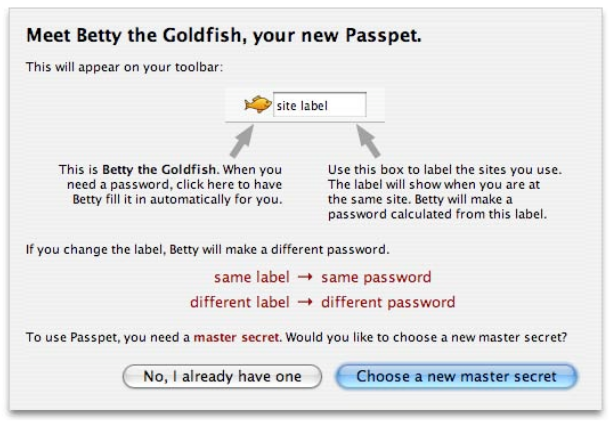
\includegraphics[width=0.95\textwidth]{figures/analysis/passpet_persona.png}
				\caption{Creation of a Passpet persona. \textbf{Source:} \cite[p.4]{passpet}.}
				\label{fig:passepet_persona}
			\end{figure}

			\begin{figure}[htbp]
				\centering
				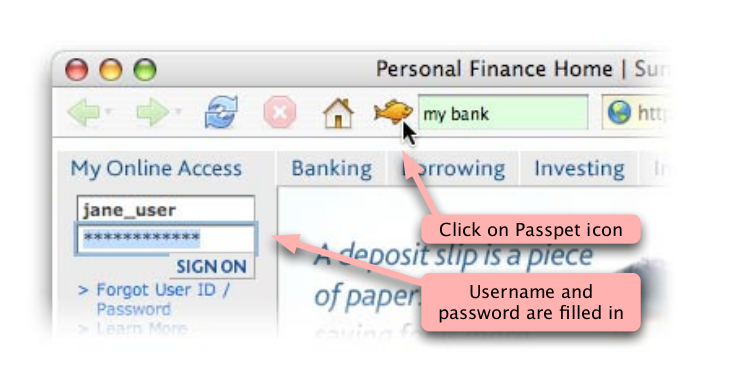
\includegraphics[width=0.95\textwidth]{figures/analysis/passpet.png}
				\caption{Using Passpet. \textbf{Source:} \cite[p.1]{passpet}}
				\label{fig:passpet_main}
			\end{figure}

			Unfortunately, there is an ambiguity in the paper. Several places, a ``Passpet server'' is mentioned, however it is never specifically told who owns this server. 

			To access passwords on other devices, the user will have to input the master address and master secret, and the remote machine will store the constants along with the label list, in order to recreate the passwords. Their description of how a user is authenticated for a second device is poorly described.

			This solution suffers from the same basic issue as described in section \ref{subsec:in-browser}: It only works for website logins, and only in the browser the plugin supports. This, combined with the ambiguity of their report leads to the conclusion that their solution is unfit to solve the problem at hand.


		\subsection*{Cloud Based Manager Using Privacy-Preserved Biometrics}
			Most solutions examined so far, has had the same approach to storing these password databases: Protect them behind a master password. In \cite{busch2014}, however, they argue for another approach: Use biometrics for authenticating access. Building on the prior work of Jain, Nandakumar, and Nagar, they employ Biometric Template Protection, to ensure that the original biometric characteristic can not be reverse engineered. This is then used, to authenticate to the cloud, containing the passwords.


			While this idea \emph{novel}, the usability is limited by our current technology. It is simply a fact, that not all of our devices are equipped with sensors able to detect biometric characteristics. Additionally, there have been voiced some concerns about using biometrics for authentication. All in all, the usage of their solution is not suitable for the problem at hand.

		\subsection*{A Password Manager that Doesn’t Remember Passwords}
			In \cite{stobert2014} another take a password manager is described. In it, they design and implement a prototype of the software Versipass. Much like the previous section, Veripass has a novel take on authenticating the user, in order to access the password database.

			Existing as a bookmarklet, Veripass presents the user with an image cue, to verify the user. In short, an image cue is a image based password. An image is divided up into a $6x8$ squares \emph{(default settings)}. A password is then a selection of these squares. An example of this, is seen on figure \ref{fig:versipass_imagecue} on page \pageref{fig:versipass_imagecue}. The squares are chosen at random, by the system. The use of randomly assigned squares, is done to avoid what they call hotspots in the images, which essentially is areas of a picture which is more likely to be chosen by users, than other areas. 

			In order to go from a set of squares into a text-based password, each tile is assigned a a string. These strings are then concatenated into a single string, in a fixed order. The resulting string is then salted and hashed, which then returns the password. In contrast to popular approach, the salt in this process is \emph{ partially user selected}. The salt consists of a combination of the sites URL and a user selected salt. This is done in order for the user to be able to change the password for a site, should it be required.

			From a security perspective, there are some shady aspects of their paper. In section 5.1.1 they cite that 21 bits of ``entropy'' is sufficient for an online attack,and quotes \cite{florencio2014}. However, there is a much more frightening problem: Combinations. In their default settings they state that a $5x6$ grid in which 5 tiles are to be selected, in any order, is sufficient. However, ignoring the advanced analysis

			Applying some math, it is evident that there exists $1712304$ different combinations using these settings, cf. equation \ref{eq:combinations}. At first glance this might seem decent, but in fact it offers \emph{less} combinations than a randomly selected $6$ character long password, consisting \emph{only} of lower-case letters, cf. equation \ref{eq:permutations}. While they do say, that the settings suggested them can be altered to increase security, it still feels like a less secure approach.

			\begin{equation}
				c = \frac{n!}{(n-r)!(r!)} = \frac{48!}{(48-5)!(5!)} = 1712304
				\label{eq:combinations}
			\end{equation}

			\begin{equation}
				p = n^r = 11881376
				\label{eq:permutations}
			\end{equation}

			\begin{figure}[htbp]
				\centering
				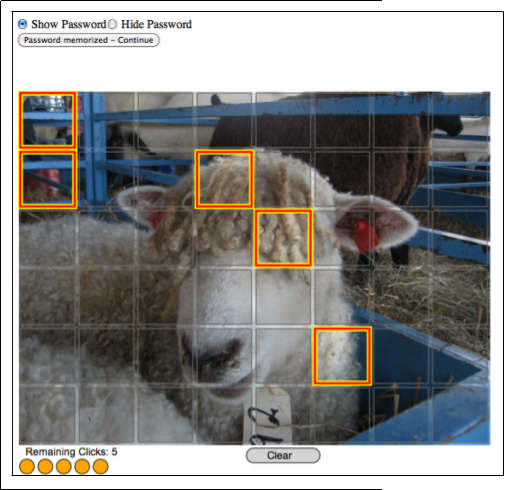
\includegraphics[width=0.95\textwidth]{figures/analysis/versipass_imagecue.png}
				\caption{Versipass' image cue password. \textbf{Source:} \cite[p.3]{stobert2014}.}
				\label{fig:versipass_imagecue}
			\end{figure}

			Abstracting away from some of the details, this solution is sort of a parallel to the one described in \cite{busch2014}. While the mechanism for unlocking the password is novel, it is just impractical. Hence, it is deemed as an unsuitable solution for the problem at hand.

		\subsection*{Password Management Using Doodles}
			Much in line with the previously described solutions, \cite{doodles} describes a novel take on the password manager. Their idea is to use doodles to log into websites.

			The basic concept is the same as has been seen over and over again; Username, passwords, and site URLs are stored in a database. Accessing these usernames and passwords, requires the user to draw his or her master doodle in a supplied browser plugin, seen on figure \ref{fig:doodle}. If this entered doodle then is a match with a stored ``master doodle'', the username and password is autofilled.

			Unfortunately, they do not disclose how exactly the database is protected. Additionally, the paper makes no effort taking multiple devices into account. As such, their solution is dismissed.

			\begin{figure}[htbp]
				\centering
				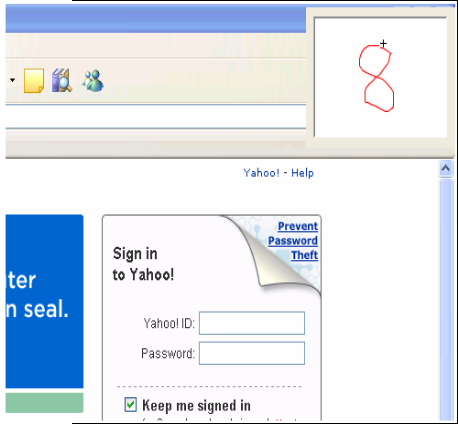
\includegraphics[width=0.95\textwidth]{figures/analysis/doodle.png}
				\caption{The Doodle browser plugin}
				\label{fig:doodle}
			\end{figure}

		\subsection*{Other Sources}
			In \cite{halderman2005} they discuss deriving site specific passwords, from a single master password and a site URL. This is done by hashing the concatenated strings, and the resulting hash is then the password for that specific site. This is a solution very similar to the one described in \cite{pwdhash}.

			In \cite{zhang2015} they have some of the same thoughts, as in \cite{pwdhash}, using a dedicated key to signal TrustLogin that confidential information is being entered. However, it differs from PwdHash as TrustLogin does not actually \emph{store} anything. It is ``merely'' a tool for secure input, on a possibly insecure platform. While their paper doesn't describe a password manager as seen previously, it does presents some interesting takes on securing the input of the user.

			In \cite{englert2009} they describe a very classical password management system: An HTTP server and a browser client. The client logs into the server, gets the encrypted data, and decrypts it locally. However, from their description of the system, the encryption key -- or as they call it the ``secret key'' -- is something the user is supposed to remember and input \emph{per} session. 

			\cite{huang2015} describes what they call a Searchable Conditional Proxy Re-Encryption scheme. Their solution, CloudKeyBank, is based on this SC-PRE scheme is claimed to not only guarantee confidentiality and privacy of the users keys, but also ensuring the privacy in regards to other attributes to each key, amongst others. However, part of their assumptions is the use of a CloudKeyBank provider, i.e. a third party, much like services such as LastPass. As such, their solution is primarily focussed on ensuring that no other person than the owner, can access data even when uploaded to third party servers.